%\documentclass[fleqn]{article}
\documentclass{article}
\usepackage{mathtools,tabu,float,hyperref,color,amsmath,amsxtra,amssymb,latexsym,amscd,amsthm,amsfonts,graphicx,enumitem,multirow,datetime}
%\usepackage{showframe}
% \numberwithin{equation}{section}
\usepackage[a4paper,left=3cm,right=3cm,top=3cm,bottom=3cm]{geometry}
\usepackage{tikz,graphicx}
\usepackage{caption}
\captionsetup[figure]{labelformat=empty}
\captionsetup[table]{labelformat=empty}
\usetikzlibrary{shapes,arrows}
\usetikzlibrary{calc}
\usetikzlibrary{decorations.pathmorphing}
%\usepackage{fancyhdr}
%\pagestyle{fancy}
%\fancyhf{}
%\fancyhead[RE,LO]{\footnotesize \textsc \rightmark}
%\cfoot{\thepage}
%\renewcommand{\headrulewidth}{0.5pt}
%\setcounter{tocdepth}{10}
%\usepackage{imakeidx}
%\makeindex[columns=2, title=Alphabetical Index, options= -s index.ist]
%\setlength{\mathindent}{0pt}
%\usepackage[utf8x]{vietnam}
\usepackage[english]{babel}

\newtheorem{theorem}{Theorem}[subsection]
\newtheorem{definition}[theorem]{Definition}
\newtheorem{proposition}[theorem]{Proposition}
\newtheorem{lemma}[theorem]{Lemma}
\newtheorem{corollary}{Corollary}[theorem]
%\addto{\renewcommand\proofname{Proof}}

\begin{document}
	\title{Finite Volume Method\\Practical Assignment}
	%\author{Đoàn Trần Nguyên Tùng\\
	%	Student ID: 1411352}
	%\selectlanguage{english}
	\author{Doan Tran Nguyen Tung\\
		Student ID: 1411352}
	\maketitle
	\tableofcontents
	\newpage
	\begin{center}
		\begin{Huge}
			Practical Assignment
		\end{Huge}
	\end{center}

	\noindent Given a 1D Poisson problem on $\Omega=(0,1)$
	\begin{equation}\label{PE1}
	-u''(x)=f(x), x\in\Omega
	\end{equation}

	\begin{enumerate}[leftmargin=*]
		\item Dirichlet boundary condition
		\begin{enumerate}[leftmargin=*,label=\alph*)]
			\item Solve the equation \eqref{PE1} subjected to homogeneous Dirichlet boundary condition
			\begin{equation}
			u(0)=a, u(1)=b
			\end{equation}
			by finite volume method on a regular grid and the control points are the midpoints of the control volumes $\left(x_i=\dfrac{x_{i-\frac{1}{2}}+x_{i+\frac{1}{2}}}{2}\right)$.

			\item Solve the equation \eqref{PE1} with regular grid and each control point is $\dfrac{1}{3}$ from the left of each control volume $\left(x_i=\frac{2}{3}x_{i-\frac{1}{2}}+\frac{1}{3}x_{i+\frac{1}{2}}\right)$

			\item How to approximate the mean value of $f$ over the control volumes $T_i$ and compare some ways of approximation.

			\item Solve the equation \eqref{PE1} with a singular grid.
		\end{enumerate}

		\item Neumann boundary condition\\
		Solve the equation \eqref{PE1} subjected to Neumann boundary condition
		\begin{equation}
		u'(0)=0, u'(1)=0 \mbox{ with } \int_{0}^{1}f(x)dx=0 \mbox{ and } \int_{0}^{1}u(x)dx=0
		\end{equation}
		by finite volume method on a regular grid and a singular grid and the control points are the midpoints of the control volumes $\left(x_i=\dfrac{x_{i-\frac{1}{2}}+x_{i+\frac{1}{2}}}{2}\right)$.
	\end{enumerate}
	\newpage
	\noindent
	\section{Dirichlet boundary condition}
	In this section, we are going to test the Finite Volume Method for the 1-dimensional Poisson equation subjected to Dirichlet boundary condition with several test cases using uniform grid and singular grid, varying positions of control points, ways of integration approximation.
	\subsection{Test cases}
	\noindent$\bullet$ \underline{Case 1:}
	\begin{flalign*}
	f(x)&=\frac{1}{2}-x&\\
	u(0)&=\frac{1}{24}&\\
	u(1)&=-\frac{1}{24}&\\
	u(x)&=\frac{x^2\,\left(2\,x-3\right)}{12}+\frac{1}{24}
	\end{flalign*}

	\noindent$\bullet$ \underline{Case 2:}
	\begin{flalign*}
	f(x)&=-20000\,x^3+\frac{957200\,x^2}{33}-\frac{1240655\,x}{99}+\frac{916835}{594}&\\
	u(0)&=-\frac{175}{44}&\\
	u(1)&=\frac{2660}{297}&\\
	u(x)&=\left(1000\,x-50\right)\,\left(x-\frac{3}{11}\right)\,\left(x-\frac{7}{9}\right)\,\left(x-\frac{5}{12}\right)\,\left(x-\frac{9}{10}\right)
	\end{flalign*}

	\noindent$\bullet$ \underline{Case 3:}
	\begin{flalign*}
	f(x)=&3\,{\cos\left(x+\frac{1}{2}\right)}^3\,{\sin\left(10\,\pi \,{\left(x+\frac{1}{2}\right)}^5\right)}^5+12500\pi^2{\cos\left(x+\frac{1}{2}\right)}^3\,{\sin\left(10\,\pi \,{\left(x+\frac{1}{2}\right)}^5\right)}^5\,{\left(x+\frac{1}{2}\right)}^8
	\\&-6\,\cos\left(x+\frac{1}{2}\right)\,{\sin\left(x+\frac{1}{2}\right)}^2\,{\sin\left(10\,\pi \,{\left(x+\frac{1}{2}\right)}^5\right)}^5
	\\&-50000\pi^2,{\cos\left(x+\frac{1}{2}\right)}^3\,{\cos\left(10\,\pi \,{\left(x+\frac{1}{2}\right)}^5\right)}^2\,{\sin\left(10\,\pi \,{\left(x+\frac{1}{2}\right)}^5\right)}^3\,{\left(x+\frac{1}{2}\right)}^8
	\\&-1000\,\pi \,{\cos\left(x+\frac{1}{2}\right)}^3\,\cos\left(10\,\pi \,{\left(x+\frac{1}{2}\right)}^5\right)\,{\sin\left(10\,\pi \,{\left(x+\frac{1}{2}\right)}^5\right)}^4\,{\left(x+\frac{1}{2}\right)}^3
	\\&+1500\,\pi \,{\cos\left(x+\frac{1}{2}\right)}^2\,\cos\left(10\,\pi \,{\left(x+\frac{1}{2}\right)}^5\right)\,\sin\left(x+\frac{1}{2}\right)\,{\sin\left(10\,\pi \,{\left(x+\frac{1}{2}\right)}^5\right)}^4\,{\left(x+\frac{1}{2}\right)}^4&\\
	u(0)=&{\sin\left(\frac{5\pi}{16}\right)}^5\,{\cos\left(\frac{1}{2}\right)}^3&\\
	u(1)=&{\sin\left(\frac{\pi}{16}\right)}^5\,{\cos\left(\frac{3}{2}\right)}^3&\\
	u(x)=&{\sin\left(10\pi\left(x+\frac{1}{2}\right)^5\right)}^5\,{\cos\left(x+\frac{1}{2}\right)}^3
	\end{flalign*}

	\newpage
	\subsection{Homogeneous Dirichlet boundary condition, regular grid, each control point is the midpoint of corresponding control volume, integration using midpoint rule}
	\subsubsection{Figures of results}
	\noindent$\bullet$ \underline{Case 1:}
	\begin{figure}[H]
		\centering	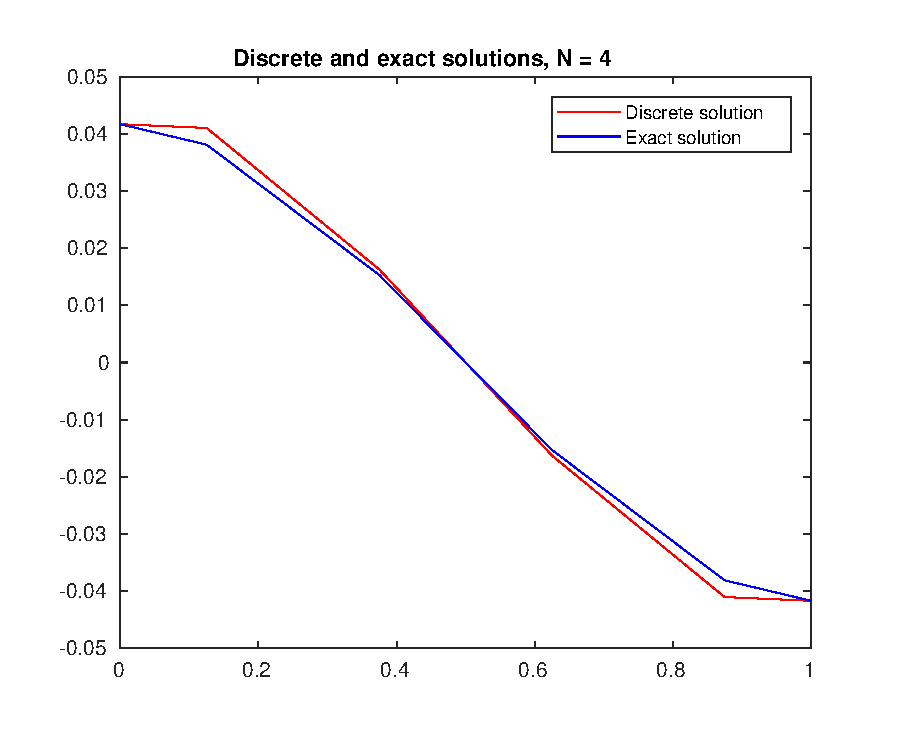
\includegraphics[width=10cm]{fig_dirichlet_result_uniform_midpoint_N4_C1}
		%%\caption{fig dirichlet result uniform midpoint N4 C1}
	\end{figure}
	\begin{figure}[H]
		\centering	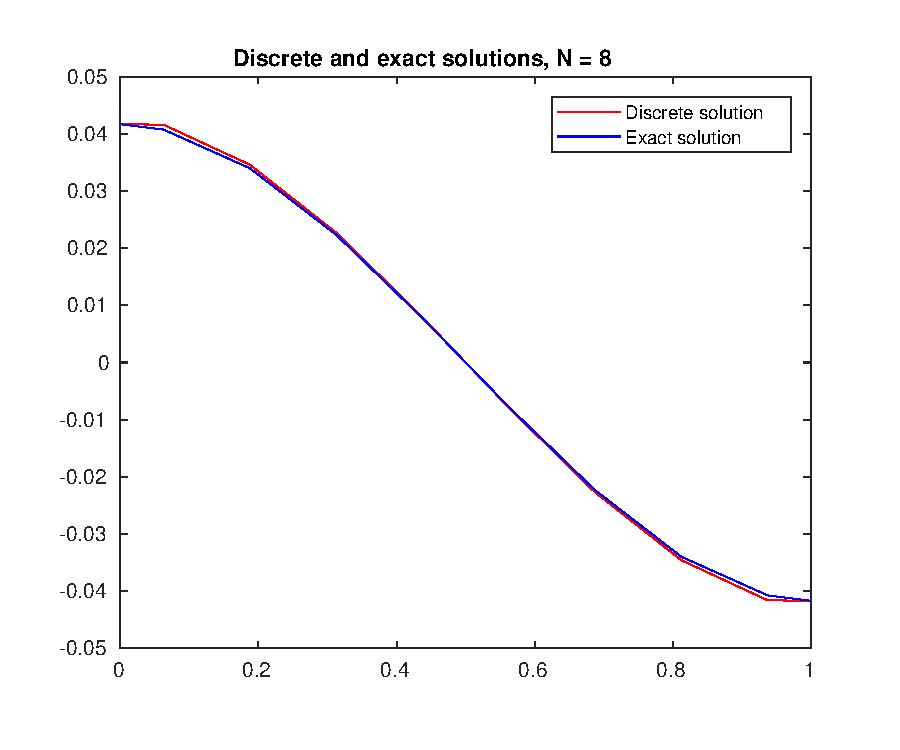
\includegraphics[width=10cm]{fig_dirichlet_result_uniform_midpoint_N8_C1}
		%%\caption{fig dirichlet result uniform midpoint N8 C1}
	\end{figure}
	\begin{figure}[H]
		\centering	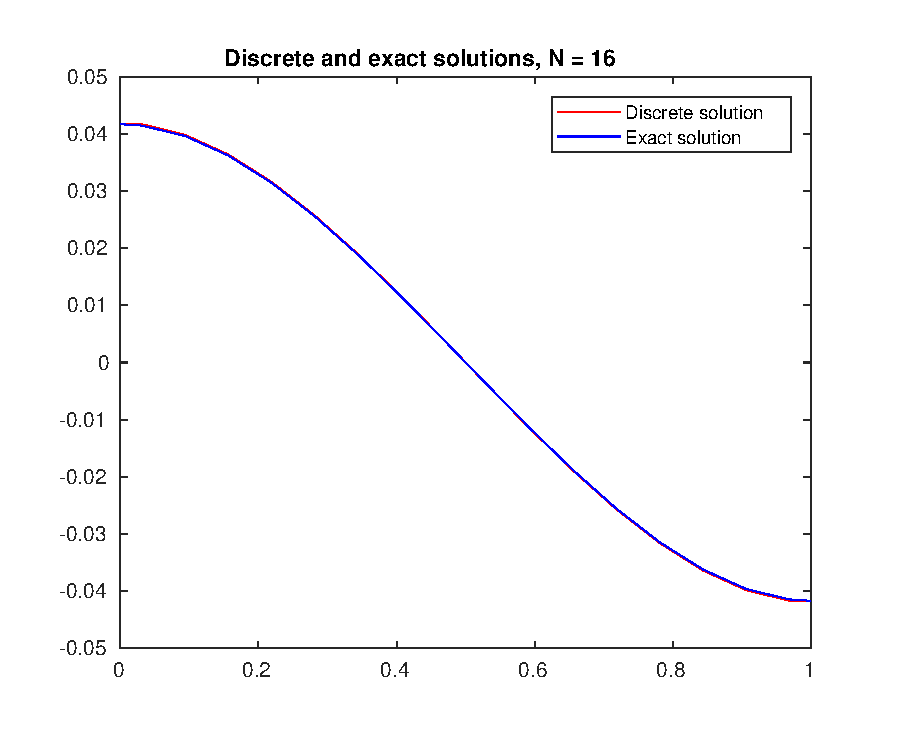
\includegraphics[width=10cm]{fig_dirichlet_result_uniform_midpoint_N16_C1}
		%%\caption{fig dirichlet result uniform midpoint N16 C1}
	\end{figure}
	\begin{figure}[H]
		\centering	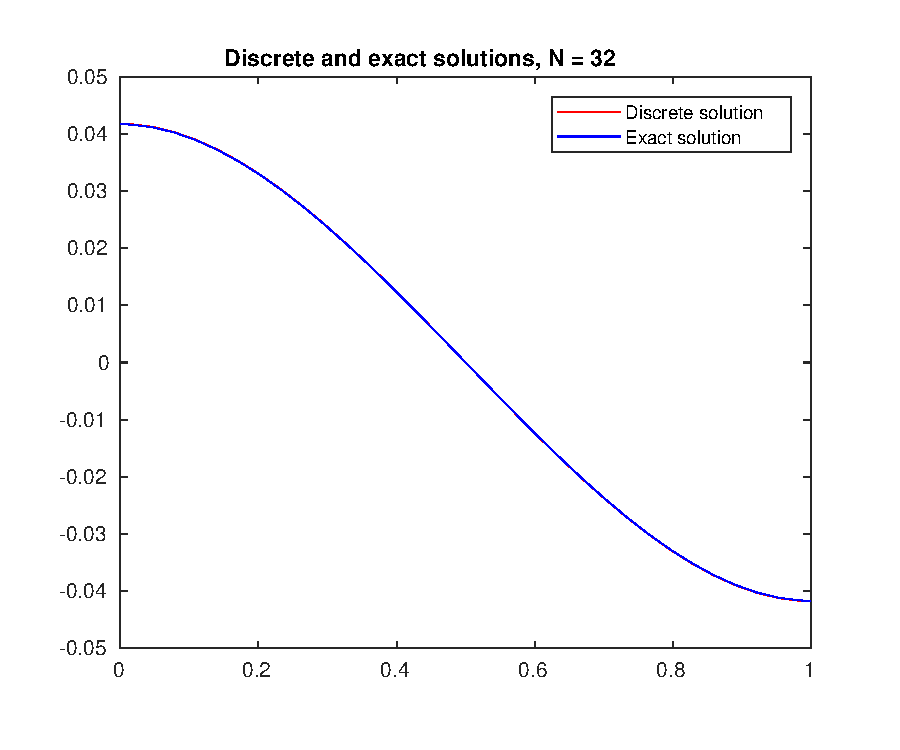
\includegraphics[width=10cm]{fig_dirichlet_result_uniform_midpoint_N32_C1}
		%%\caption{fig dirichlet result uniform midpoint N32 C1}
	\end{figure}
	\begin{figure}[H]
		\centering	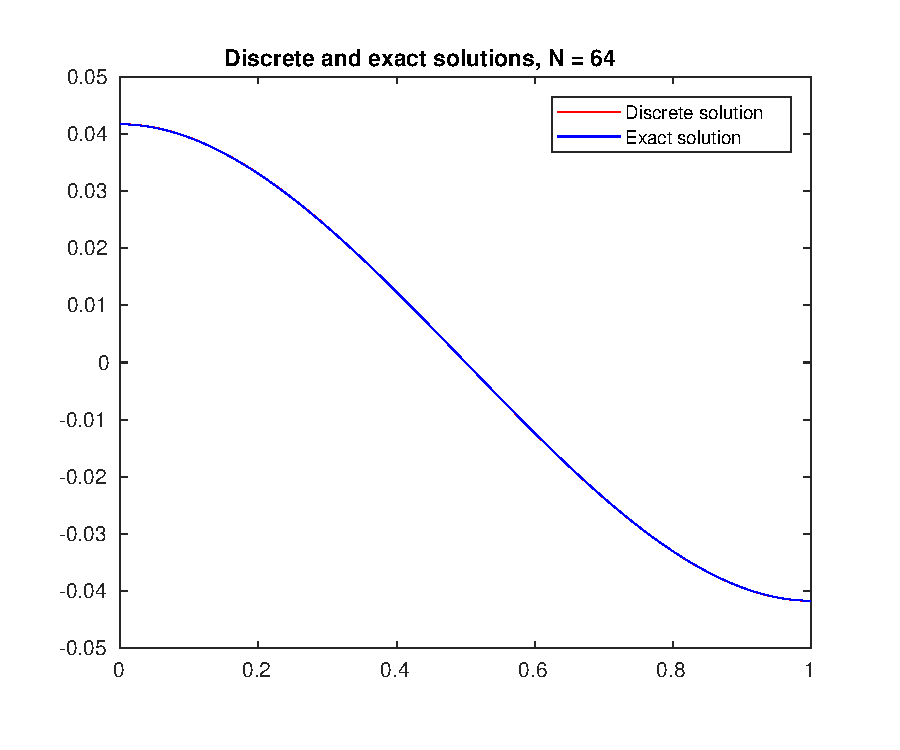
\includegraphics[width=10cm]{fig_dirichlet_result_uniform_midpoint_N64_C1}
		%%\caption{fig dirichlet result uniform midpoint N64 C1}
	\end{figure}
	\begin{figure}[H]
		\centering	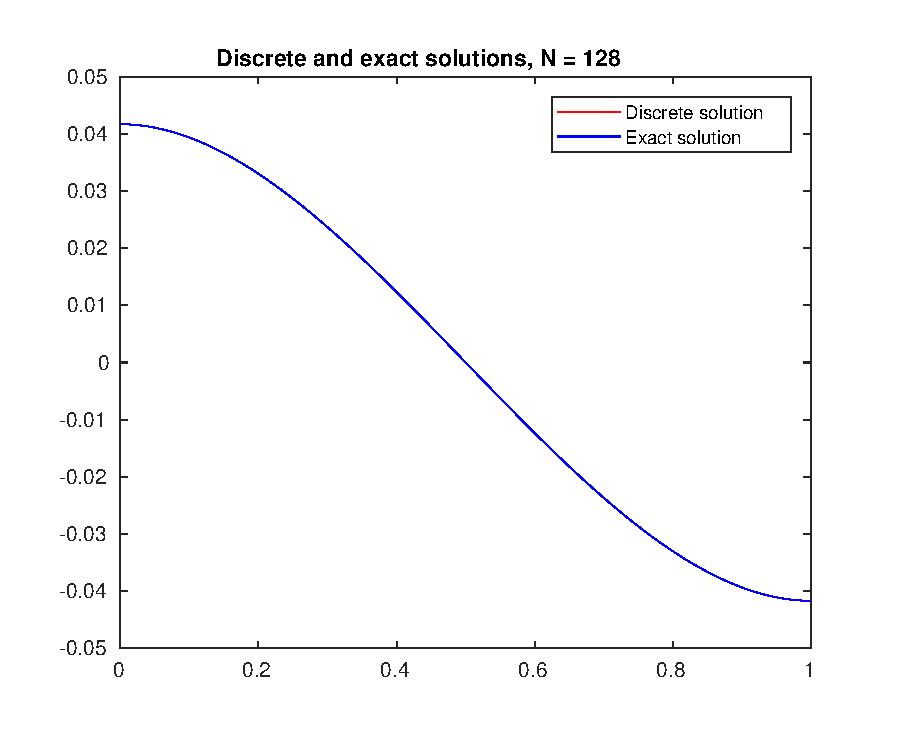
\includegraphics[width=10cm]{fig_dirichlet_result_uniform_midpoint_N128_C1}
		%%\caption{fig dirichlet result uniform midpoint N128 C1}
	\end{figure}

	\noindent$\bullet$ \underline{Case 2:}
	\begin{figure}[H]
		\centering	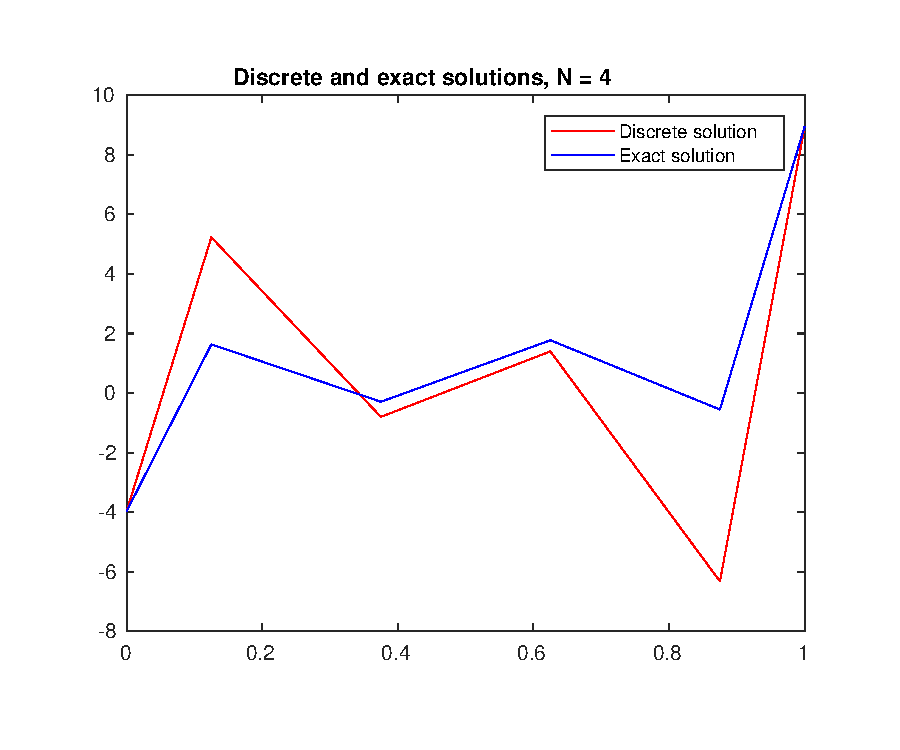
\includegraphics[width=10cm]{fig_dirichlet_result_uniform_midpoint_N4_C2}
		%%\caption{fig dirichlet result uniform midpoint N4 C2}
	\end{figure}
	\begin{figure}[H]
		\centering	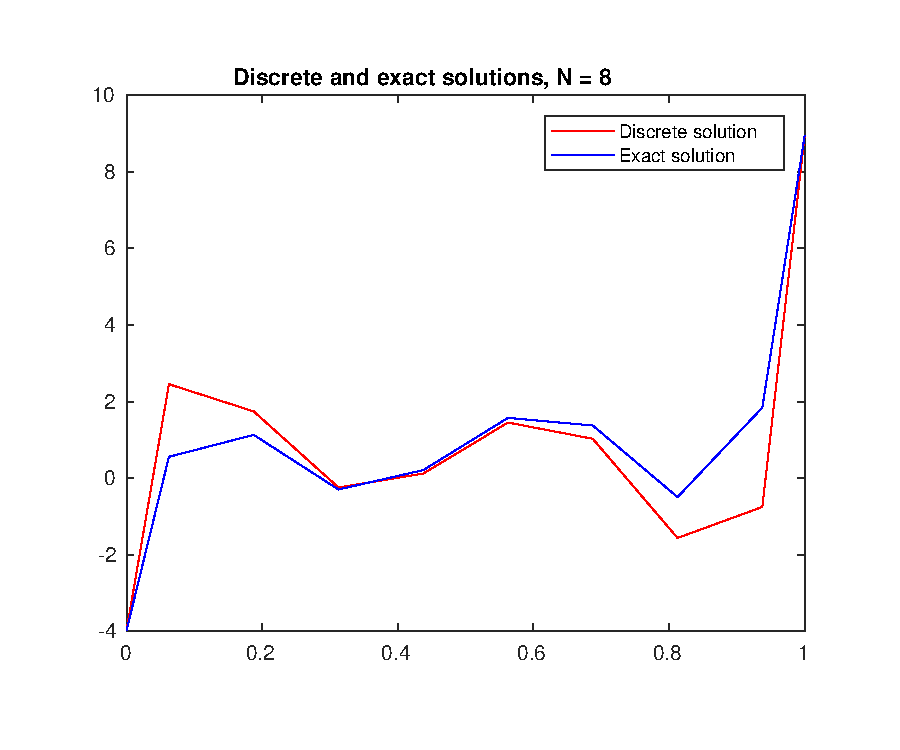
\includegraphics[width=10cm]{fig_dirichlet_result_uniform_midpoint_N8_C2}
		%%\caption{fig dirichlet result uniform midpoint N8 C2}
	\end{figure}
	\begin{figure}[H]
		\centering	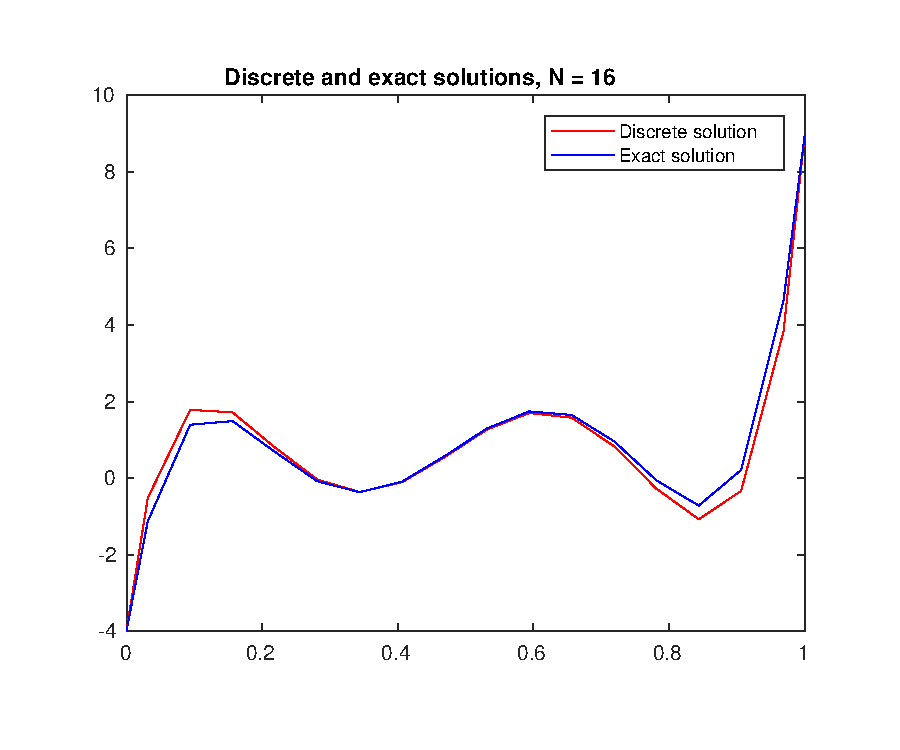
\includegraphics[width=10cm]{fig_dirichlet_result_uniform_midpoint_N16_C2}
		%%\caption{fig dirichlet result uniform midpoint N16 C2}
	\end{figure}
	\begin{figure}[H]
		\centering	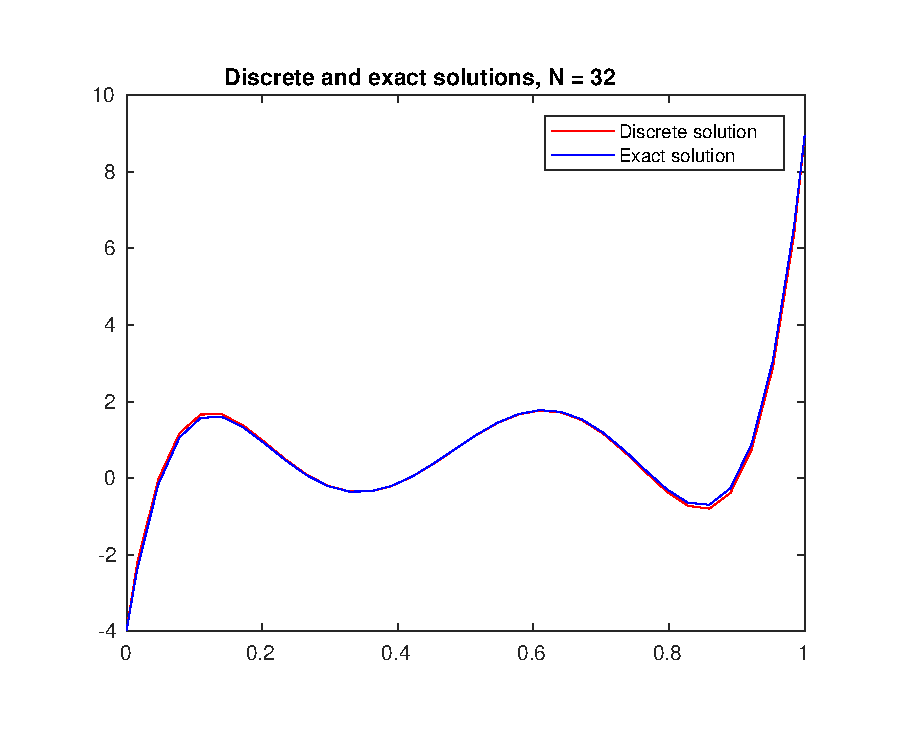
\includegraphics[width=10cm]{fig_dirichlet_result_uniform_midpoint_N32_C2}
		%%\caption{fig dirichlet result uniform midpoint N32 C2}
	\end{figure}
	\begin{figure}[H]
		\centering	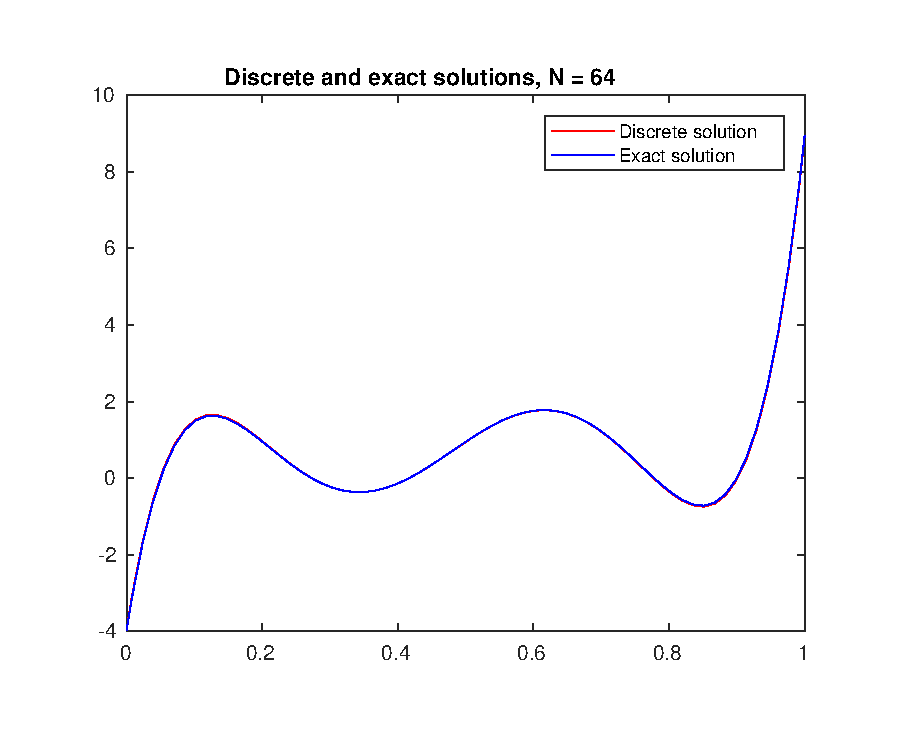
\includegraphics[width=10cm]{fig_dirichlet_result_uniform_midpoint_N64_C2}
		%%\caption{fig dirichlet result uniform midpoint N64 C2}
	\end{figure}
	\begin{figure}[H]
		\centering	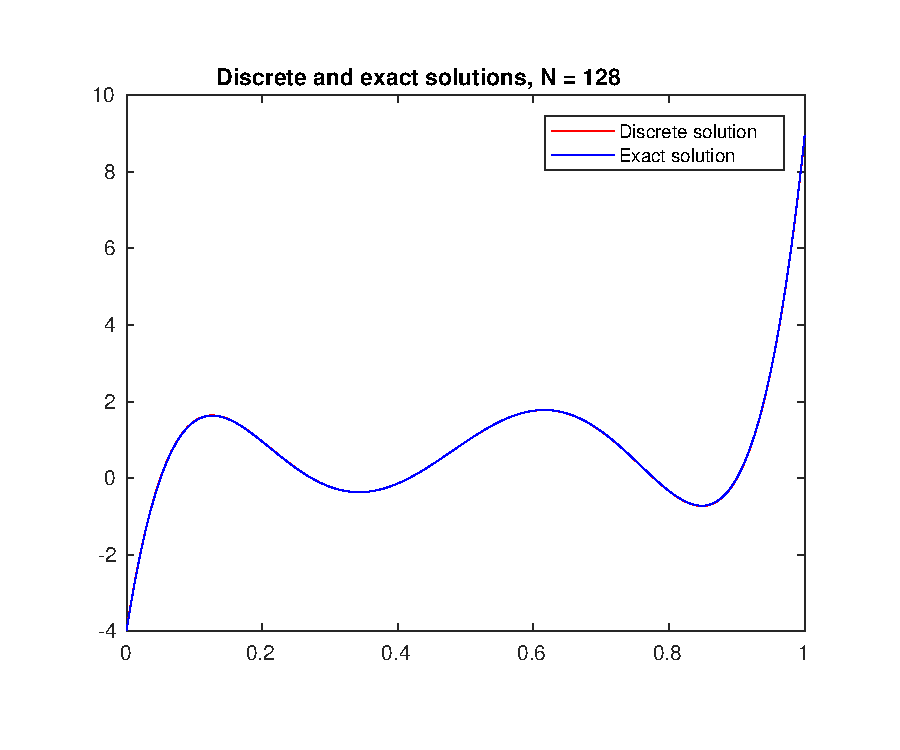
\includegraphics[width=10cm]{fig_dirichlet_result_uniform_midpoint_N128_C2}
		%%\caption{fig dirichlet result uniform midpoint N128 C2}
	\end{figure}

	\noindent$\bullet$ \underline{Case 3:}
	\begin{figure}[H]
		\centering	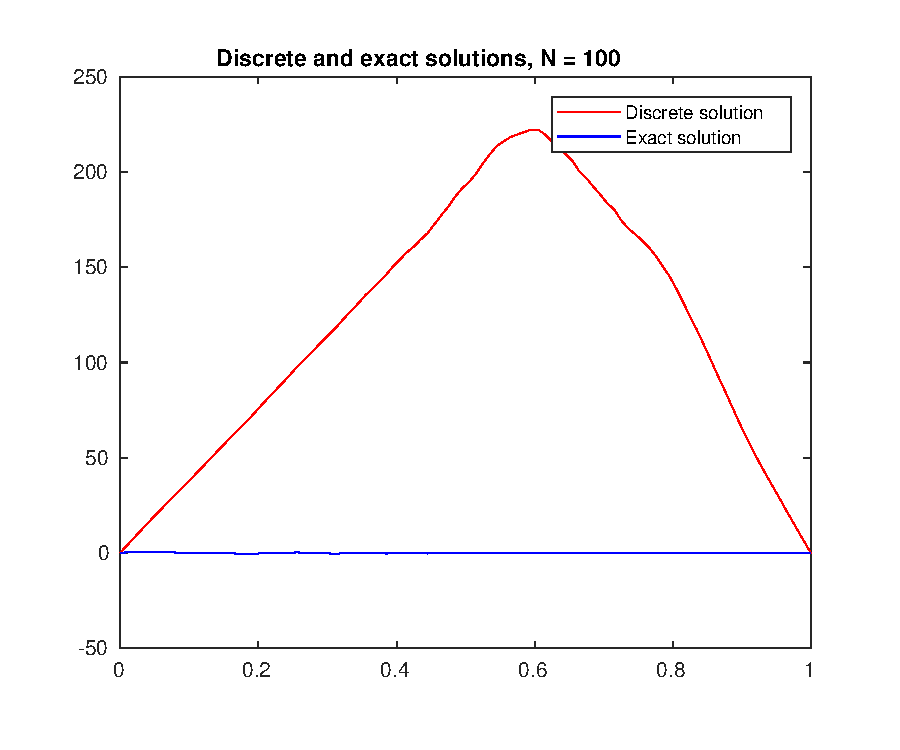
\includegraphics[width=10cm]{fig_dirichlet_result_uniform_midpoint_N100_C3}
		%%\caption{fig dirichlet result uniform midpoint N100 C3}
	\end{figure}
	\begin{figure}[H]
		\centering	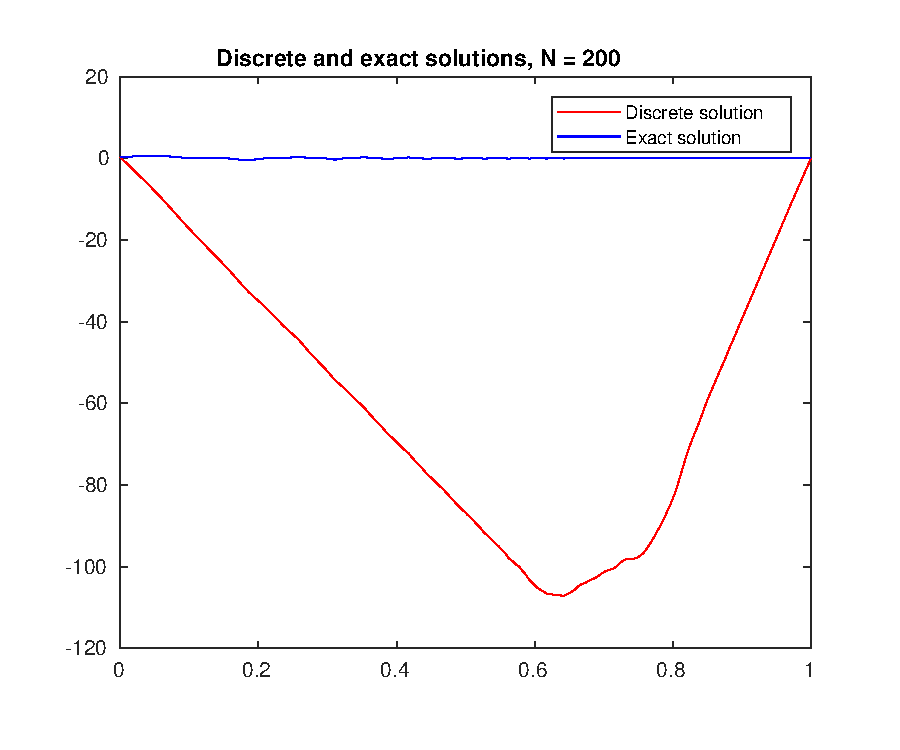
\includegraphics[width=10cm]{fig_dirichlet_result_uniform_midpoint_N200_C3}
		%%\caption{fig dirichlet result uniform midpoint N200 C3}
	\end{figure}
	\begin{figure}[H]
		\centering	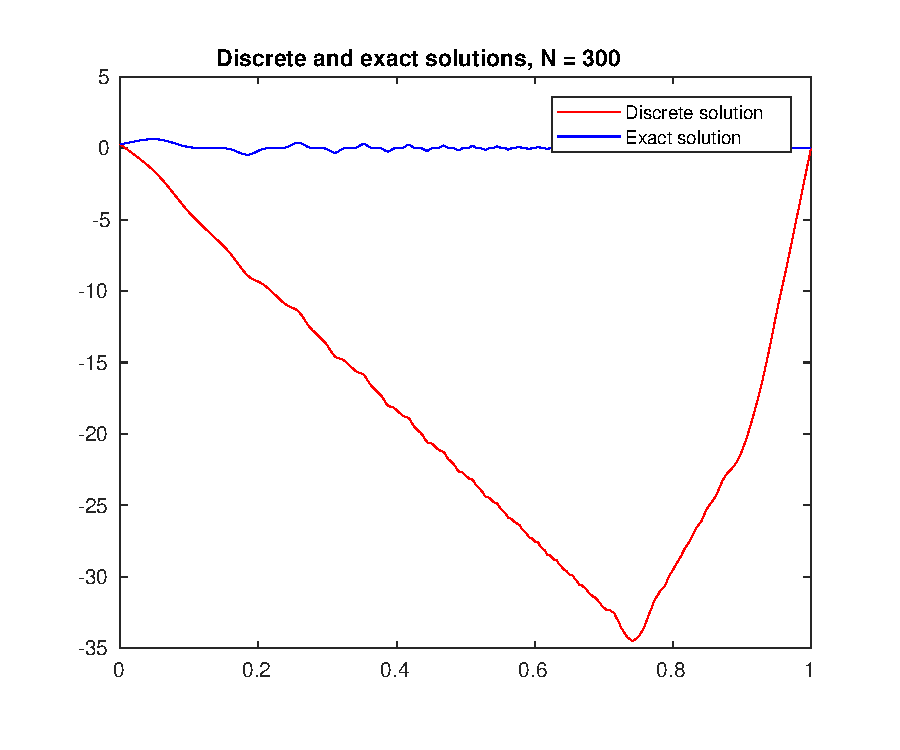
\includegraphics[width=10cm]{fig_dirichlet_result_uniform_midpoint_N300_C3}
		%%\caption{fig dirichlet result uniform midpoint N400 C3}
	\end{figure}
	\begin{figure}[H]
		\centering	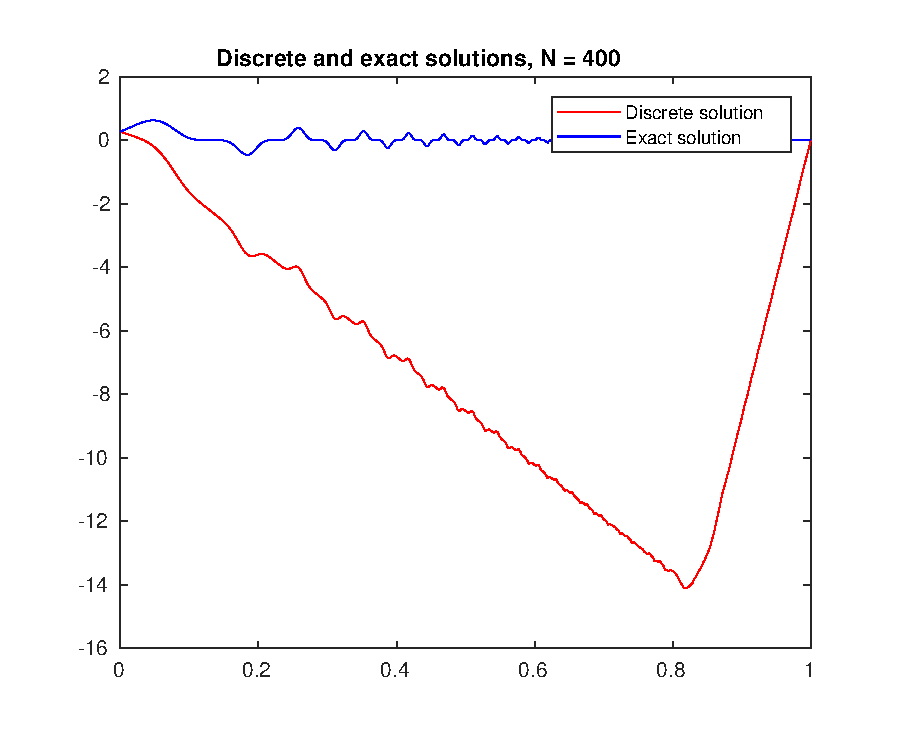
\includegraphics[width=10cm]{fig_dirichlet_result_uniform_midpoint_N400_C3}
		%%\caption{fig dirichlet result uniform midpoint N500 C3}
	\end{figure}
	\begin{figure}[H]
		\centering	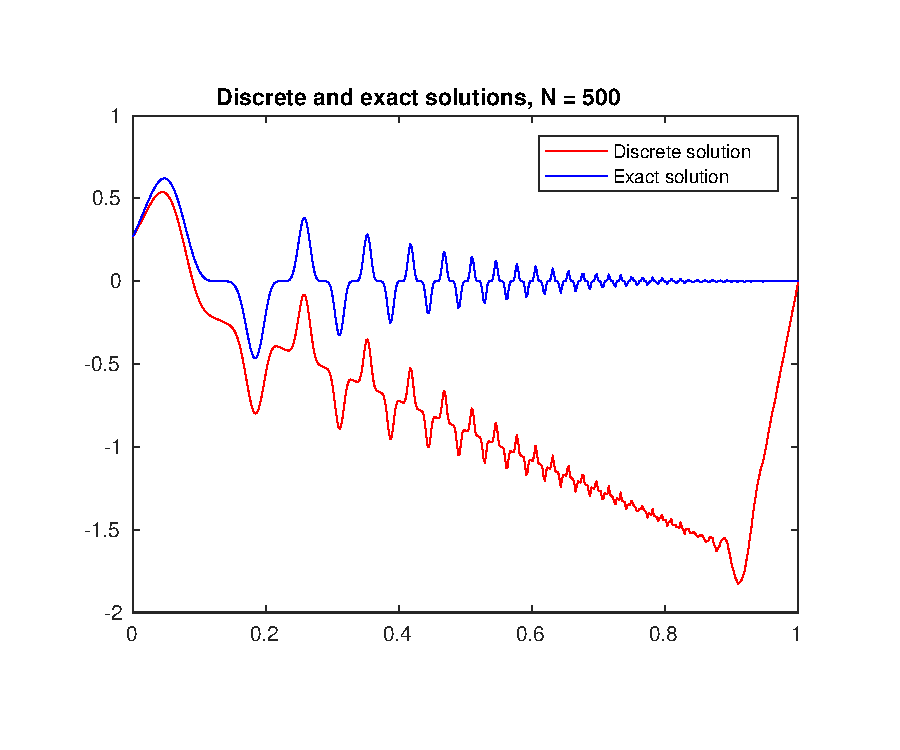
\includegraphics[width=10cm]{fig_dirichlet_result_uniform_midpoint_N500_C3}
		%%\caption{fig dirichlet result uniform midpoint N600 C3}
	\end{figure}
	\begin{figure}[H]
		\centering	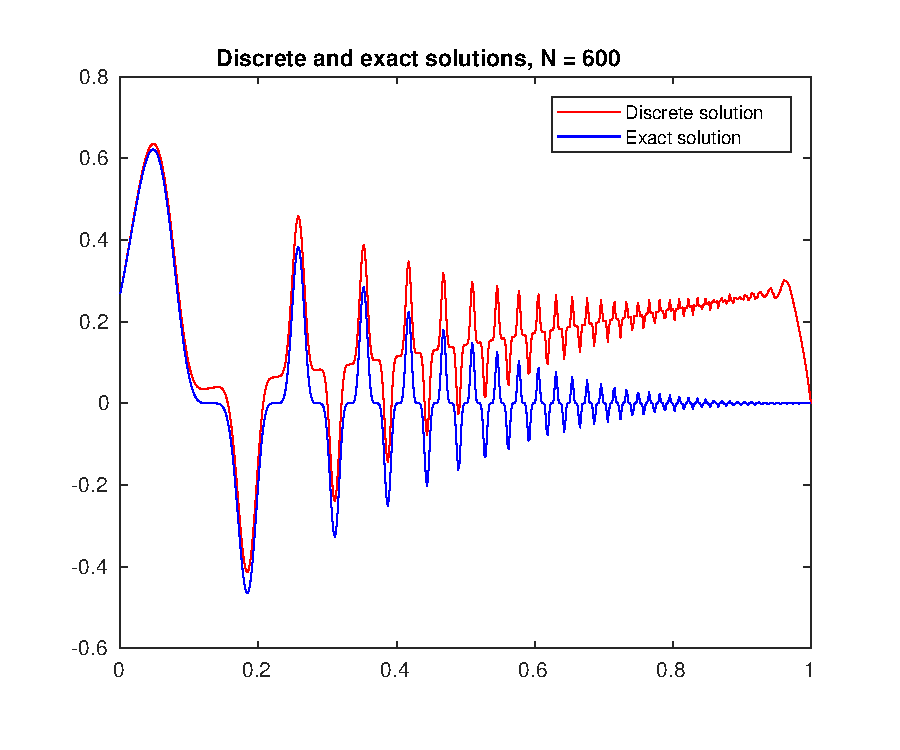
\includegraphics[width=10cm]{fig_dirichlet_result_uniform_midpoint_N600_C3}
		%%\caption{fig dirichlet result uniform midpoint N600 C3}
	\end{figure}
	\begin{figure}[H]
		\centering	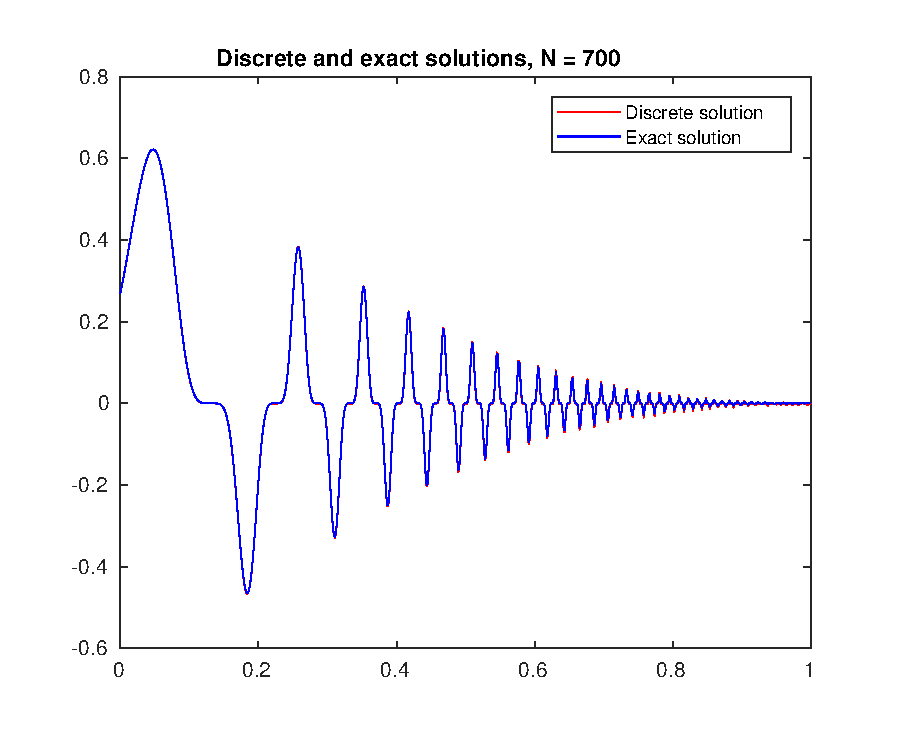
\includegraphics[width=10cm]{fig_dirichlet_result_uniform_midpoint_N700_C3}
		%%\caption{fig dirichlet result uniform midpoint N700 C3}
	\end{figure}
	\begin{figure}[H]
		\centering	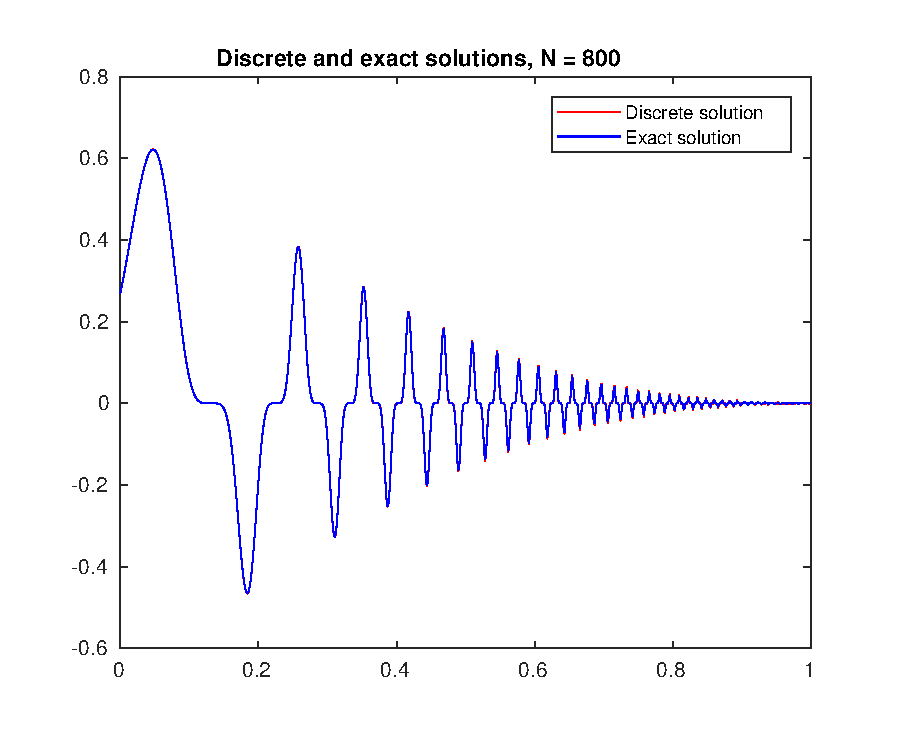
\includegraphics[width=10cm]{fig_dirichlet_result_uniform_midpoint_N800_C3}
		%%\caption{fig dirichlet result uniform midpoint N800 C3}
	\end{figure}
	\newpage
	\subsubsection{Errors}
	\noindent$\bullet$ \underline{Case 1:}
	\begin{table}[H]
		\centering
		\begin{tabu}{|c|c|c|}
			\hline
			N	&  $\lVert u_{discrete}-u_{exact}\rVert_{L^2}$& $\lVert u_{discrete}-u_{exact}\rVert_{H^1}$ \\\hline
			4	& 2.183660e-03 & 1.353165e-02 \\\hline
			8	& 5.593964e-04 & 5.167483e-03 \\\hline
			16	& 1.406791e-04 & 1.891105e-03 \\\hline
			32	& 3.522145e-05 & 6.796587e-04 \\\hline
			64	& 8.808591e-06 & 2.422258e-04 \\\hline
			128	& 2.202349e-06 & 8.597891e-05 \\\hline
		\end{tabu}
		%%\caption{Error table}
	\end{table}

	\noindent$\bullet$ \underline{Case 2:}
	\begin{table}[H]
		\centering
		\begin{tabu}{|c|c|c|}
			\hline
			N	&  $\lVert u_{discrete}-u_{exact}\rVert_{L^2}$& $\lVert u_{discrete}-u_{exact}\rVert_{H^1}$ \\\hline
			4	& 3.414525e+00 & 1.723527e-02 \\\hline
			8	& 1.224066e+00 & 1.429127e+01 \\\hline
			16	& 3.297560e-01 & 6.028506e+00 \\\hline
			32	& 8.393195e-02 & 2.295482e+00 \\\hline
			64	& 2.107644e-02 & 8.397813e-01 \\\hline
			128	& 5.274953e-03 & 3.018207e-01 \\\hline
		\end{tabu}
		%%\caption{Error table}
	\end{table}

	\noindent$\bullet$ \underline{Case 3:}
	\begin{table}[H]
		\centering
		\begin{tabu}{|c|c|c|}
			\hline
			N	&  $\lVert u_{discrete}-u_{exact}\rVert_{L^2}$& $\lVert u_{discrete}-u_{exact}\rVert_{H^1}$ \\\hline
			100	& 1.372029e+02 & 4.718806e+02 \\\hline
			200	& 6.795356e+01 & 2.432018e+02 \\\hline
			300	& 2.068556e+01 & 8.656798e+01 \\\hline
			400	& 8.220398e+00 & 3.814539e+01 \\\hline
			500	& 9.637916e-01 & 7.476626e+00 \\\hline
			600	& 1.613099e-01 & 2.708167e+00 \\\hline
			700	& 1.691419e-03 & 1.378369e+00 \\\hline
			800	& 1.035571e-03 & 1.034955e+00 \\\hline
		\end{tabu}
		%%\caption{Error table}
	\end{table}

	\newpage
	\subsubsection{Convergence rate}
	\noindent$\bullet$ \underline{Case 1:}
	\begin{figure}[H]
		\centering	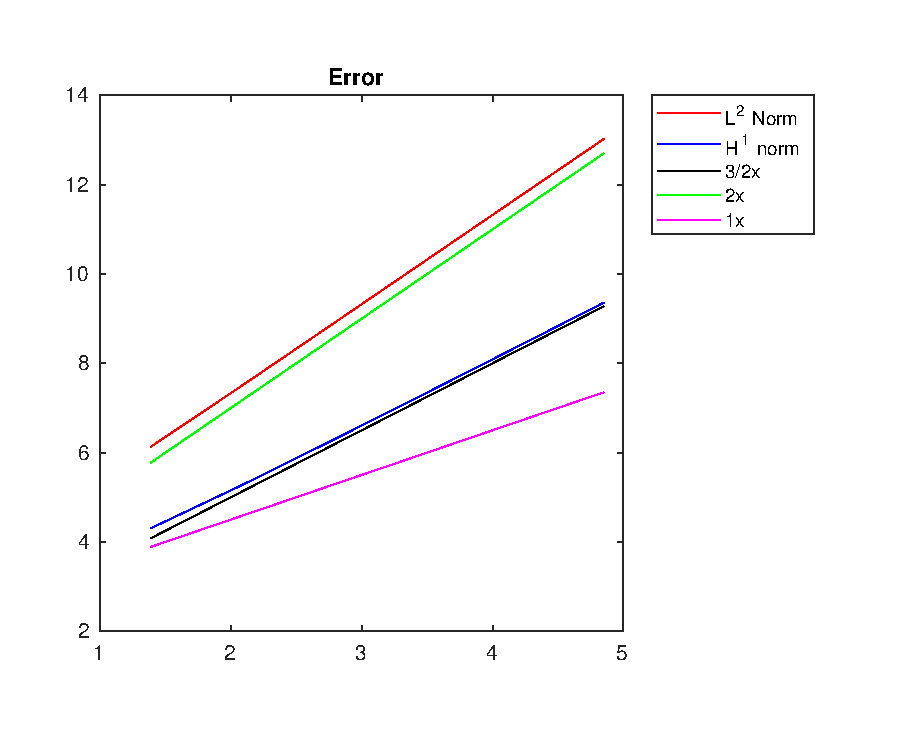
\includegraphics[width=10cm]{fig_dirichlet_error_midpoint_cp_uniform_midpoint_C1_M6}
		%%\caption{fig dirichlet error midpoint cp uniform midpoint C1 M6}
	\end{figure}

	\noindent$\bullet$ \underline{Case 2:}
	\begin{figure}[H]
		\centering	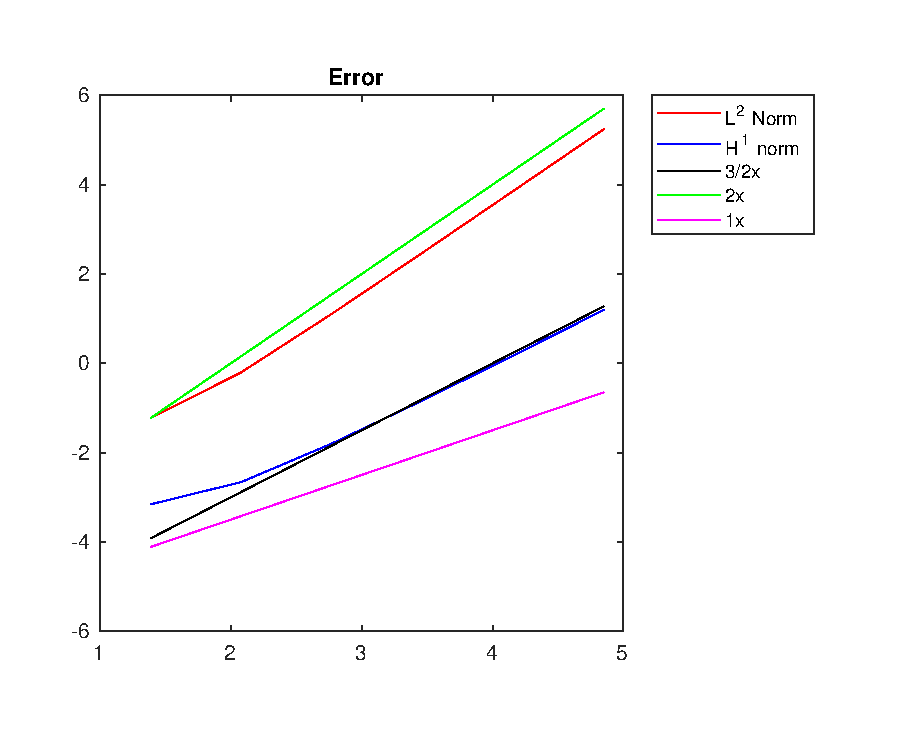
\includegraphics[width=10cm]{fig_dirichlet_error_midpoint_cp_uniform_midpoint_C2_M6}
		%%\caption{fig dirichlet error midpoint cp uniform midpoint C2 M6}
	\end{figure}
	\noindent$\bullet$ \underline{Case 3:}
	\begin{figure}[H]
		\centering	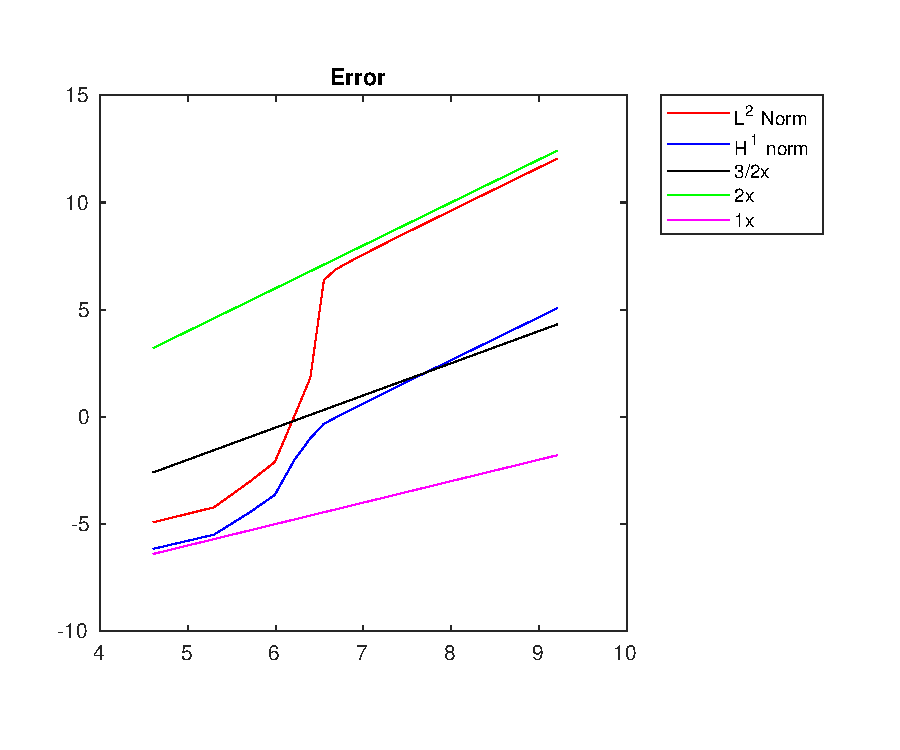
\includegraphics[width=10cm]{fig_dirichlet_error_midpoint_cp_uniform_midpoint_C3_M100}
		%%\caption{fig dirichlet error midpoint cp uniform midpoint C3 M100}
	\end{figure}
	\noindent\textbf{Remark:} We can see that in case 1 and 2, the finite volume method has convergence rate of order $2$ in $L^2$ norm and order $\frac{3}{2}$ in energy norm. But in case 3, finite volume method has convergence rate of order $2$ in both $L^2$ and energy norm. More ever, the convergence rate in case 3 only become consistent after the grid refinement reached a certain degree.
	\newpage
	\subsection{Homogeneous Dirichlet boundary condition, regular grid, each control point is 1/3 from the left of corresponding control volume, integration using midpoint rule}
	\subsubsection{Errors}
	\noindent$\bullet$ \underline{Case 1:}
	\begin{table}[H]
		\centering
		\begin{tabu}{|c|c|c|}
			\hline
			N	&  $\lVert u_{discrete}-u_{exact}\rVert_{L^2}$& $\lVert u_{discrete}-u_{exact}\rVert_{H^1}$ \\\hline
			4	& 4.337732e-03 & 1.723527e-02 \\\hline
			8	& 1.976011e-03 & 7.696433e-03 \\\hline
			16	& 9.604458e-04 & 3.489791e-03 \\\hline
			32	& 4.766545e-04 & 1.633552e-03 \\\hline
			64	& 2.378772e-04 & 7.855739e-04 \\\hline
			128	& 1.188822e-04 & 3.845069e-04\\\hline
		\end{tabu}
		%%\caption{Error table}
	\end{table}

	\noindent$\bullet$ \underline{Case 2:}
	\begin{table}[H]
		\centering
		\begin{tabu}{|c|c|c|}
			\hline
			N	&  $\lVert u_{discrete}-u_{exact}\rVert_{L^2}$& $\lVert u_{discrete}-u_{exact}\rVert_{H^1}$ \\\hline
			4	& 6.063755e+00 & 2.989757e+01 \\\hline
			8	& 3.072003e+00 & 1.824323e+01 \\\hline
			16	& 1.453481e+00 & 8.493182e+00\\\hline
			32	& 7.060401e-01 & 3.804418e+00\\\hline
			64	& 3.484227e-01 & 1.738566e+00 \\\hline
			128	& 1.731597e-01 & 8.193746e-01\\\hline
		\end{tabu}
		%%\caption{Error table}
	\end{table}

	\noindent$\bullet$ \underline{Case 3:}
	\begin{table}[H]
		\centering
		\begin{tabu}{|c|c|c|}
			\hline
			N	&  $\lVert u_{discrete}-u_{exact}\rVert_{L^2}$& $\lVert u_{discrete}-u_{exact}\rVert_{H^1}$ \\\hline
			100	& 1.374387e+02 & 4.724692e+02 \\\hline
			200	& 6.805998e+01 & 2.434741e+02 \\\hline
			300	& 2.074894e+01 & 8.685629e+01 \\\hline
			400	& 8.237658e+00 & 3.826618e+01 \\\hline
			500	& 9.680948e-01 & 7.883261e+00 \\\hline
			600	& 1.628207e-01 & 3.371928e+00 \\\hline
			700	& 4.196379e-03 & 2.193966e+00 \\\hline
			800	& 3.381889e-03 & 1.786729e+00 \\\hline
		\end{tabu}
		%%\caption{Error table}
	\end{table}

	\newpage
	\subsubsection{Convergence rate}
	\noindent\underline{Case 1:}
	\begin{figure}[H]
		\centering	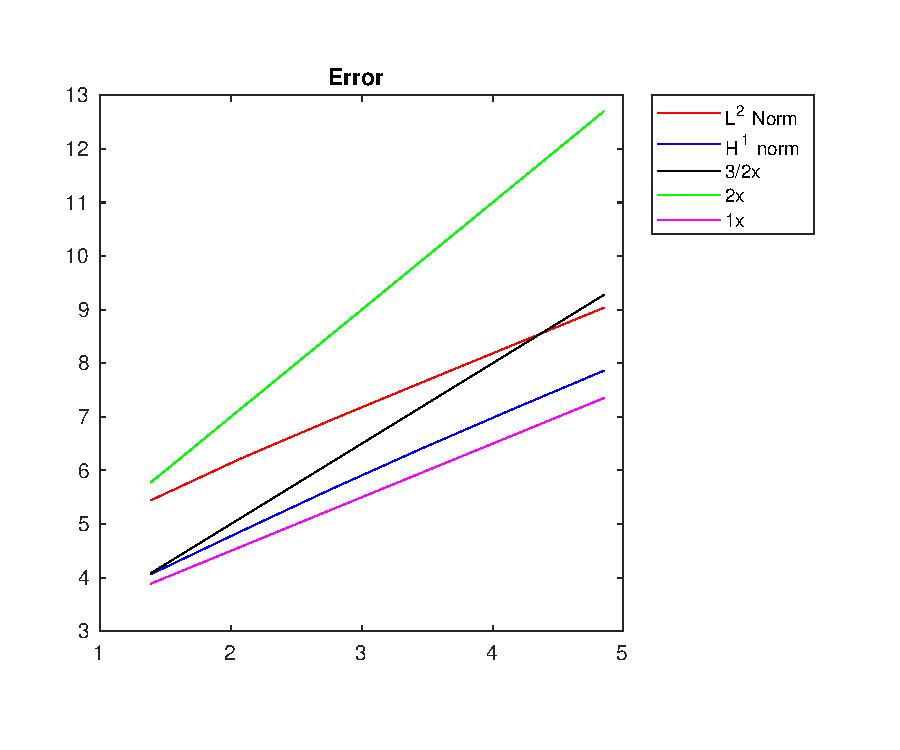
\includegraphics[width=10cm]{fig_dirichlet_error_left_cp_uniform_midpoint_C1_M6}
		%%\caption{fig dirichlet error left cp uniform midpoint C1 M6}
	\end{figure}

	\noindent$\bullet$ \underline{Case 2:}
	\begin{figure}[H]
		\centering	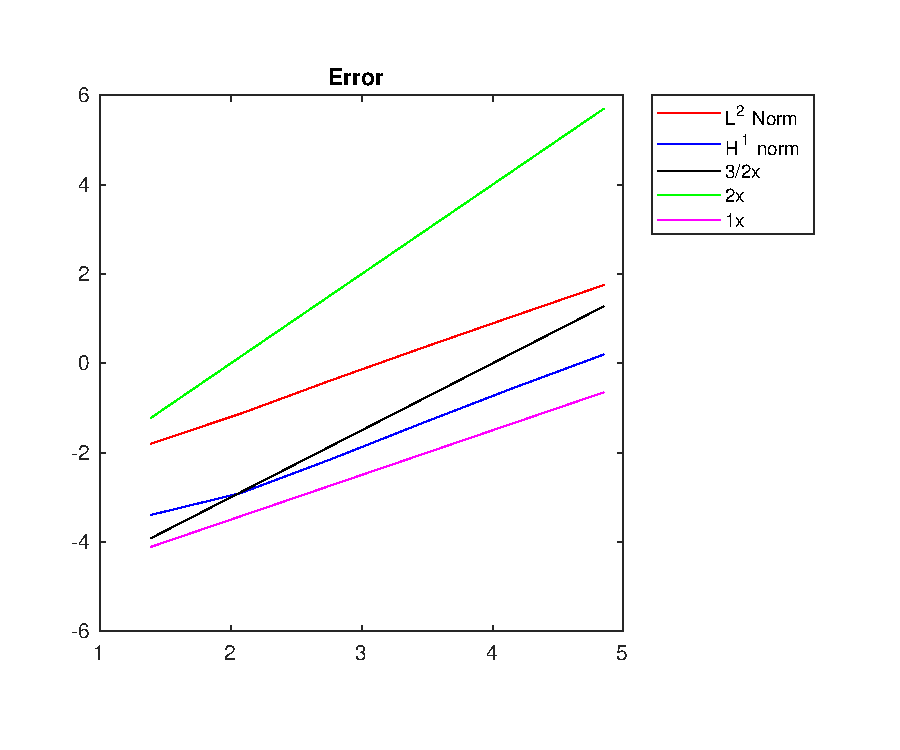
\includegraphics[width=10cm]{fig_dirichlet_error_left_cp_uniform_midpoint_C2_M6}
		%%\caption{fig dirichlet error left cp uniform midpoint C2 M6}
	\end{figure}

	\noindent$\bullet$ \underline{Case 3:}
	\begin{figure}[H]
		\centering	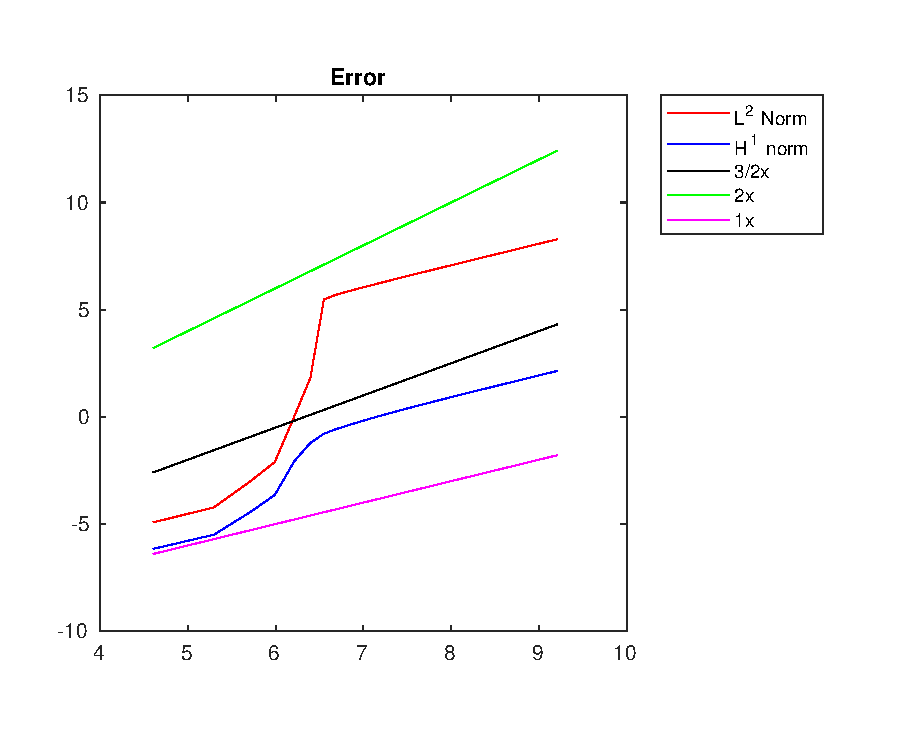
\includegraphics[width=10cm]{fig_dirichlet_error_left_cp_uniform_midpoint_C3_M100}
		%%\caption{fig dirichlet error left cp uniform midpoint C3 M100}
	\end{figure}
	\noindent\textbf{Remark:} Unlike the results in previous section, in all 3 cases, the finite volume method has convergence rate of order $1$ in both $L^p$ and energy norm. However, in case 3, similar to before, the convergence rate in case 3 only become consistent after the grid refinement reached a certain degree.
	\newpage

	\subsection{Ways to approximate the mean value of the function f over control volumes}
	\subsubsection{Somes way to approximate integral}
	There are many ways to approximate integrals, both with equally spaced integration points and unequally spaced integration points. However, we are going to test only a few way of approximation with equally spaced integration points.\\
	We need to approximate $\frac{1}{x_{i+\frac{1}{2}}-x_{i-\frac{1}{2}}}\int_{x_{i-\frac{1}{2}}}^{x_{i+\frac{1}{2}}}f(x)$, with $T_i=\left[x_{i-\frac{1}{2}},x_{i+\frac{1}{2}}\right]$ being the control volume on which we need to approximate the mean value of $f$. For the sake of convenience, let $a=x_{i-\frac{1}{2}}$ and $b=x_{i+\frac{1}{2}}$.\\
	\noindent\textbf{Midpoint rule}\\
	\begin{flalign*}
		\frac{1}{b-a}\int_{a}^{b}f(x)&=\frac{1}{b-a}(b-a)f\left(\frac{a+b}{2}\right)-\frac{1}{b-a}\frac{(b-a)^3}{24}f^{(2)}(\xi)&\\
		&=f\left(\frac{a+b}{2}\right)-\frac{(b-a)^2}{24}f^{(2)}(\xi)
	\end{flalign*}
	For some $\xi$ in $[a,b]$.\\
	\noindent\textbf{Trapezoidal rule}\\
	\begin{flalign*}
	\frac{1}{b-a}\int_{a}^{b}f(x)&=\frac{1}{b-a}\frac{b-a}{2}(f(a)+f(b))-\frac{1}{b-a}\frac{1}{12}(b-a)^3f^{(2)}(\xi)&\\
	&=\frac{f(a)+f(b)}{2}-\frac{1}{12}(b-a)^2f^{(2)}(\xi)
	\end{flalign*}
	For some $\xi$ in $[a,b]$.\\
	\noindent\textbf{Simpson's rule}\\
	Let $h=\frac{b-a}{2}$, $t_1=a$, $t_2=a+h=\frac{b-a}{2}$, $t_3=a+2h=b$.
	\begin{flalign*}
	\frac{1}{b-a}\int_{a}^{b}f(x)&=\frac{1}{2h}\frac{1}{3}\left(f(t_1)+4f(t_2)+f(t_3)\right)+\frac{1}{2h}\frac{1}{90}h^5f^{(4)}(\xi)&\\
	&=\frac{1}{6h}\left(f(t_1)+4f(t_2)+f(t_3)\right)+\frac{1}{180}h^4f^{(4)}(\xi)
	\end{flalign*}
	For some $\xi$ in $[a,b]$.\\
	\noindent\textbf{Boole's rule}\\
	Let $h=\frac{b-a}{4}$, $t_1=a$, $t_2=a+h$, $t_3=a+2h$, $t_4=a+3h$, $t_5=a+4h=b$.
	\begin{flalign*}
	\frac{1}{b-a}\int_{a}^{b}f(x)&=\frac{1}{4h}\frac{2}{45}h\left(7f(t_1)+32f(t_2)+12f(t_3)+32f(t_4)+7f(t_5)\right)-\frac{8}{945}h^7f^{(6)}(\xi)&\\
	&=\frac{1}{90}h\left(7f(t_1)+32f(t_2)+12f(t_3)+32f(t_4)+7f(t_5)\right)-\frac{8}{945}h^7f^{(6)}(\xi)&
	\end{flalign*}
	For some $\xi$ in $[a,b]$.
	\subsubsection{Effects in the Finite Volume Method}
	In this section, we will test case 3 with various methods of integration.
	\noindent\textbf{Errors}\\
	\noindent$\bullet$ \underline{Case 3:}
	\begin{table}[H]
		\centering
		\begin{tabu}{|c|c|c|}
			\hline
			N	&  $\lVert u_{discrete}-u_{exact}\rVert_{L^2}$& $\lVert u_{discrete}-u_{exact}\rVert_{H^1}$ \\\hline
			100	& 1.372029e+02 & 4.718806e+02 \\\hline
			200	& 6.795356e+01 & 2.432018e+02 \\\hline
			300	& 2.068556e+01 & 8.656798e+01 \\\hline
			400	& 8.220398e+00 & 3.814539e+01 \\\hline
			500	& 9.637916e-01 & 7.476626e+00 \\\hline
			600	& 1.613099e-01 & 2.708167e+00 \\\hline
			700	& 1.691419e-03 & 1.378369e+00 \\\hline
			800	& 1.035571e-03 & 1.034955e+00 \\\hline
		\end{tabu}
		\caption{Error table - Midpoint rule}
	\end{table}

	\begin{table}[H]
		\centering
		\begin{tabu}{|c|c|c|}
			\hline
			N	&  $\lVert u_{discrete}-u_{exact}\rVert_{L^2}$& $\lVert u_{discrete}-u_{exact}\rVert_{H^1}$ \\\hline
			100	& 3.773644e+01 & 2.412211e+02 \\\hline
			200	& 8.391778e+01 & 3.030967e+02 \\\hline
			300	& 2.038450e+01 & 8.486880e+01 \\\hline
			400	& 8.220498e+00 & 3.799774e+01 \\\hline
			500	& 9.637879e-01 & 7.212178e+00 \\\hline
			600	& 1.612986e-01 & 2.251598e+00 \\\hline
			700	& 1.234248e-03 & 8.617033e-01 \\\hline
			800	& 5.799255e-04 & 6.097104e-01 \\\hline
		\end{tabu}
		\caption{Error table - Trepozoidal rule}
	\end{table}

	\begin{table}[H]
		\centering
		\begin{tabu}{|c|c|c|}
			\hline
			N	&  $\lVert u_{discrete}-u_{exact}\rVert_{L^2}$& $\lVert u_{discrete}-u_{exact}\rVert_{H^1}$ \\\hline
			100	& 1.014161e+02 & 3.530643e+02 \\\hline
			200	& 1.742818e+01 & 6.491145e+01 \\\hline
			300	& 6.995754e+00 & 2.947754e+01 \\\hline
			400	& 2.740099e+00 & 1.278054e+01 \\\hline
			500	& 3.212656e-01 & 2.611736e+00 \\\hline
			600	& 5.377526e-02 & 1.087361e+00 \\\hline
			700	& 7.420314e-04 & 6.371791e-01 \\\hline
			800	& 4.998059e-04 & 4.889503e-01 \\\hline
		\end{tabu}
		\caption{Error table - Simpson's rule}
	\end{table}

	\begin{table}[H]
		\centering
		\begin{tabu}{|c|c|c|}
			\hline
			N	&  $\lVert u_{discrete}-u_{exact}\rVert_{L^2}$& $\lVert u_{discrete}-u_{exact}\rVert_{H^1}$ \\\hline
			100	& 2.543855e+01 & 9.312152e+01 \\\hline
			200	& 1.936562e+00 & 1.267931e+01 \\\hline
			300	& 5.423098e-01 & 3.614971e+00 \\\hline
			400	& 1.670127e-01 & 1.894852e+00 \\\hline
			500	& 3.154194e-02 & 1.063986e+00 \\\hline
			600	& 1.971232e-03 & 8.160713e-01 \\\hline
			700	& 6.508166e-04 & 5.954282e-01 \\\hline
			800	& 4.865046e-04 & 4.672134e-01 \\\hline
		\end{tabu}
		\caption{Error table - Boole's rule}
	\end{table}
	\noindent\textbf{Remark:} We can see that there are some variation in the accuracy when using different integration methods. 
	
	\newpage
	\noindent\textbf{Convergence rate}\\
	\noindent$\bullet$ \underline{Case 3:}
	\noindent$M=100$
	\begin{figure}[H]
		\centering	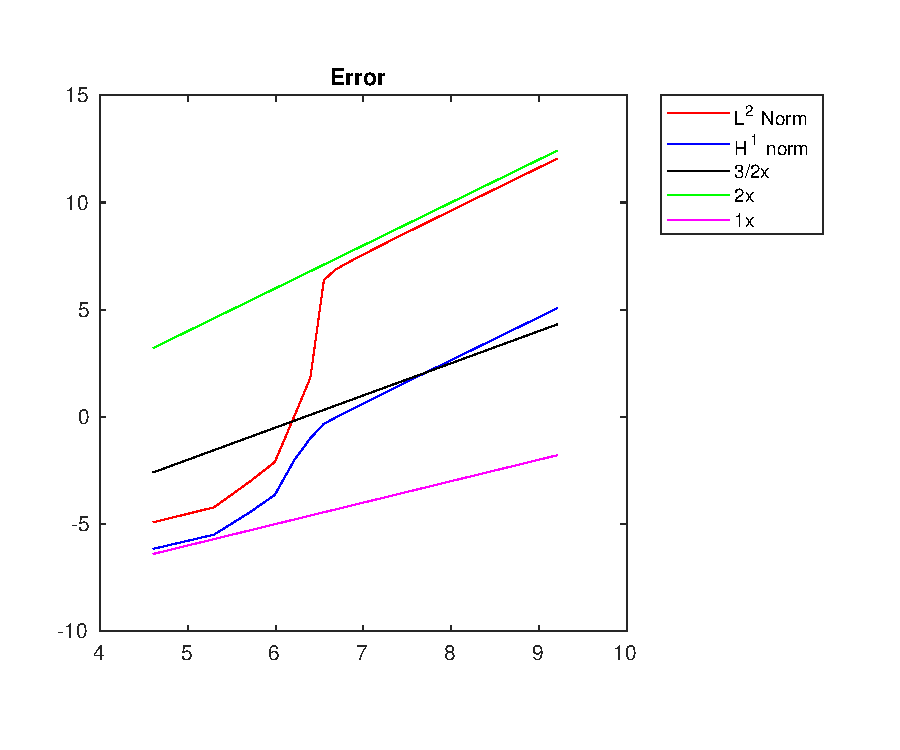
\includegraphics[width=10cm]{fig_dirichlet_error_midpoint_cp_uniform_midpoint_C3_M100}
		%%\caption{fig dirichlet error midpoint cp uniform midpoint C3 M100}
	\end{figure}

	\begin{figure}[H]
		\centering	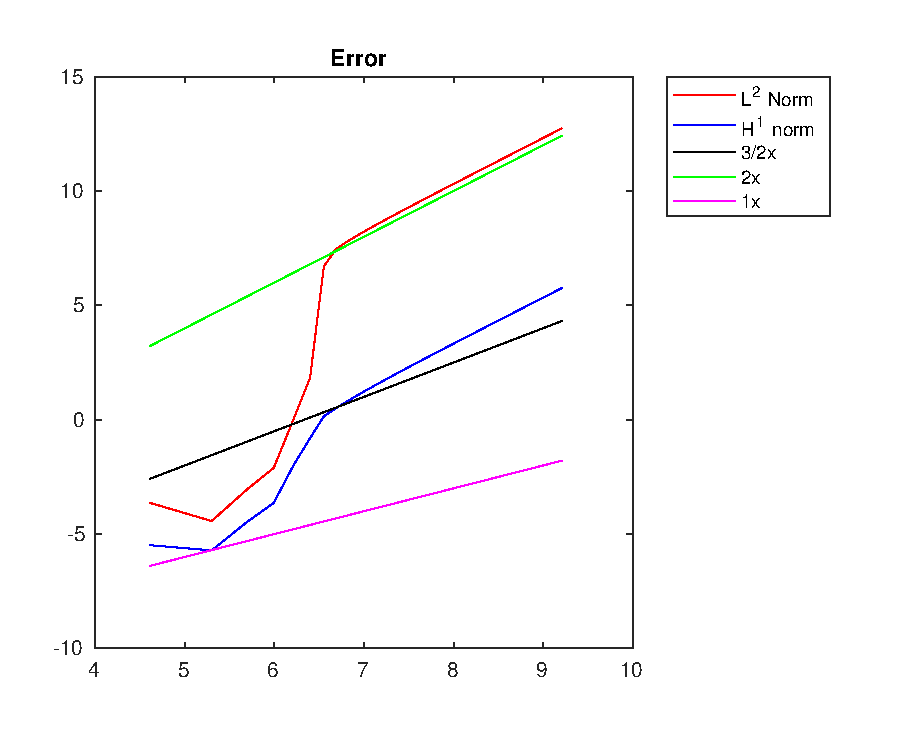
\includegraphics[width=10cm]{fig_dirichlet_error_midpoint_cp_uniform_trepozoidal_C3_M100}
		%%\caption{fig dirichlet error midpoint cp uniform trepozoidal C3 M100}
	\end{figure}

	\begin{figure}[H]
		\centering	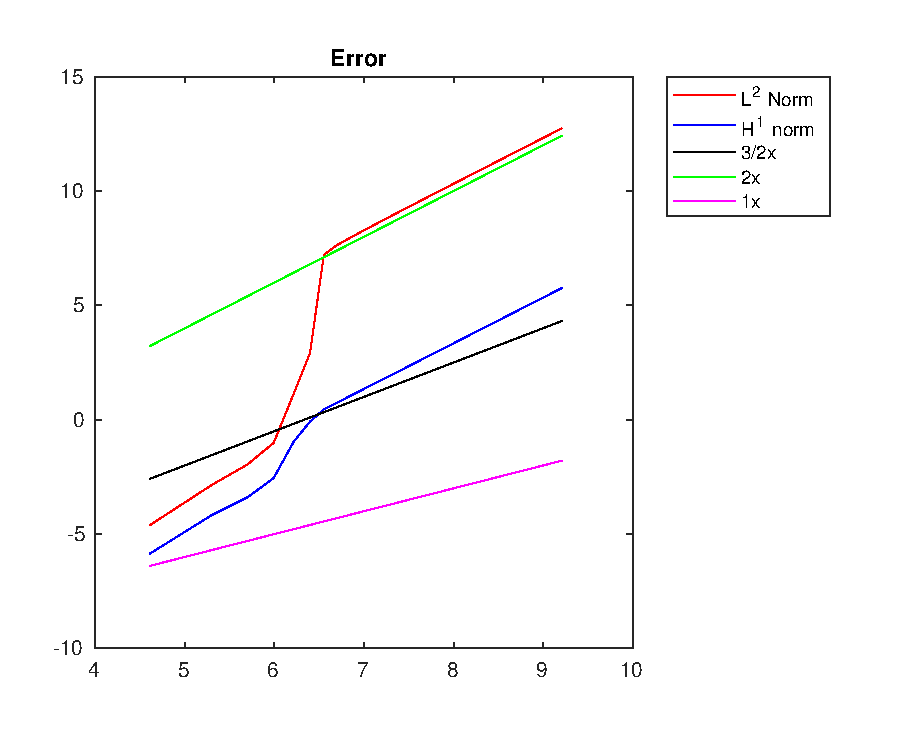
\includegraphics[width=10cm]{fig_dirichlet_error_midpoint_cp_uniform_simpson_C3_M100}
		%%\caption{fig dirichlet error midpoint cp uniform simpson C3 M100}
	\end{figure}

	\begin{figure}[H]
		\centering	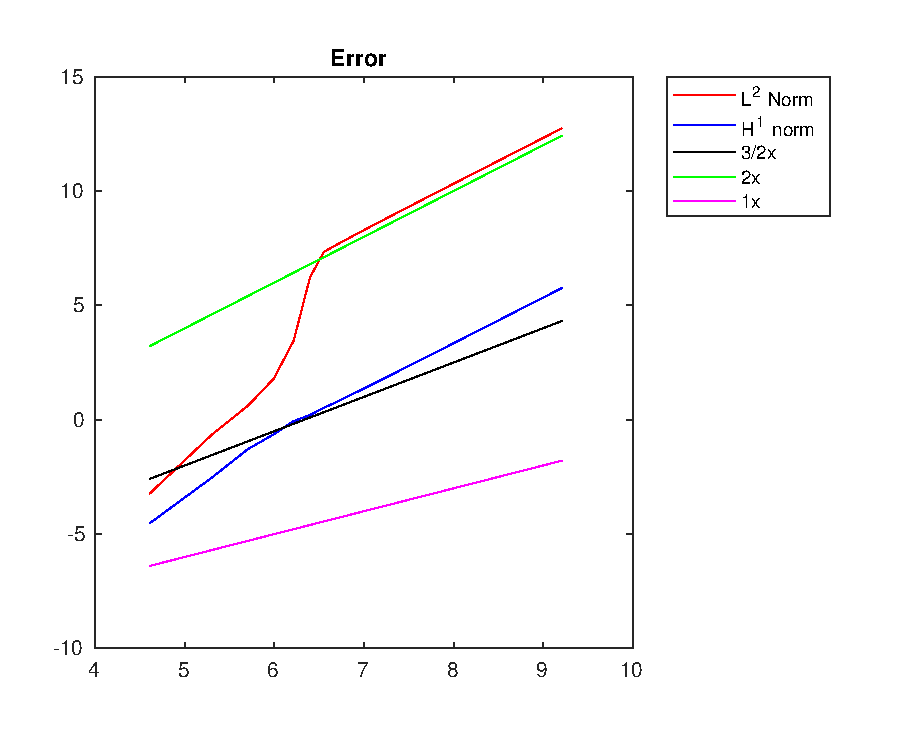
\includegraphics[width=10cm]{fig_dirichlet_error_midpoint_cp_uniform_boole_C3_M100}
		%%\caption{fig dirichlet error midpoint cp uniform boole C3 M100}
	\end{figure}

	\newpage
	\subsection{Homogeneous Dirichlet boundary condition, singular grid, each control point is the midpoint of corresponding control volume}
	In this section, we will consider the grid
	%$x_i=a+\left(1-\cos\left(\frac{\pi i}{2(N+1)}\right)\right)(b-a)$
	$x_i=1-\cos\left(\frac{\pi i}{2(N+1)}\right)$
	\subsubsection{Errors}
	\noindent$\bullet$ \underline{Case 1:}
	\begin{table}[H]
		\centering
		\begin{tabu}{|c|c|c|}
			\hline
			N	&  $\lVert u_{discrete}-u_{exact}\rVert_{L^2}$& $\lVert u_{discrete}-u_{exact}\rVert_{H^1}$ \\\hline
			4	& 2.572594e-03 & 1.408303e-02 \\\hline
			8	& 8.312800e-04 & 6.052092e-03 \\\hline
			16	& 2.366590e-04 & 2.399498e-03 \\\hline
			32	& 6.309364e-05 & 9.021918e-04 \\\hline
			64	& 1.628265e-05 & 3.291959e-04 \\\hline
			128	& 4.135350e-06 & 1.182551e-04 \\\hline
		\end{tabu}
		%%\caption{Error table}
	\end{table}

	\noindent$\bullet$ \underline{Case 2:}
	\begin{table}[H]
		\centering
		\begin{tabu}{|c|c|c|}
			\hline
			N	&  $\lVert u_{discrete}-u_{exact}\rVert_{L^2}$& $\lVert u_{discrete}-u_{exact}\rVert_{H^1}$ \\\hline
			4	& 5.147535e+00 & 2.212485e+01 \\\hline
			8	& 2.426569e+00 & 1.848306e+01 \\\hline
			16	& 7.617805e-01 & 9.789540e+00 \\\hline
			32	& 2.084740e-01 & 4.495505e+00 \\\hline
			64	& 5.417277e-02 & 2.011451e+00 \\\hline
			128	& 1.378284e-02 & 9.183423e-01 \\\hline
		\end{tabu}
		%%\caption{Error table}
	\end{table}

	\noindent$\bullet$ \underline{Case 3:}
	\begin{table}[H]
		\centering
		\begin{tabu}{|c|c|c|}
			\hline
			N	&  $\lVert u_{discrete}-u_{exact}\rVert_{L^2}$& $\lVert u_{discrete}-u_{exact}\rVert_{H^1}$ \\\hline
			100	& 2.382533e+02 & 7.816445e+02 \\\hline
			200	& 1.021832e+02 & 3.524253e+02 \\\hline
			300	& 6.461806e+01 & 2.324792e+02 \\\hline
			400	& 3.011621e+01 & 1.225957e+02 \\\hline
			500	& 2.319667e+01 & 9.540720e+01 \\\hline
			600	& 1.878345e+00 & 1.109190e+01 \\\hline
			700	& 2.656605e+00 & 1.539149e+01 \\\hline
			800	& 2.128635e+00 & 1.401007e+01 \\\hline
			900	& 2.328867e-01 & 3.282076e+00\\\hline
			1000	& 1.798795e-02 & 1.705853e+00 \\\hline
			1100	& 1.554054e-03 & 1.344722e+00 \\\hline
			1200	& 1.011087e-03 & 1.052726e+00 \\\hline
		\end{tabu}
		%%\caption{Error table}
	\end{table}

	\newpage
	\subsubsection{Convergence rate}
	\noindent$\bullet$ \underline{Case 1:}
	\begin{figure}[H]
		\centering	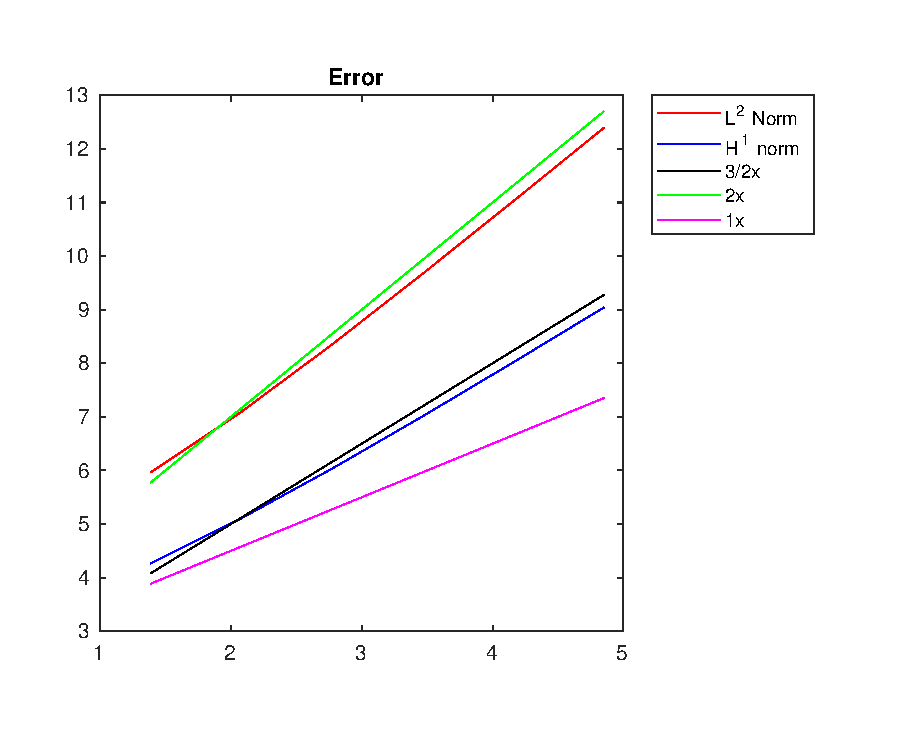
\includegraphics[width=10cm]{fig_dirichlet_error_G2_CP1_I1_M6_C1}
		%%\caption{fig dirichlet error G2 CP1 I1 M6 C1}
	\end{figure}
	\noindent$\bullet$ \underline{Case 2:}
	\begin{figure}[H]
		\centering	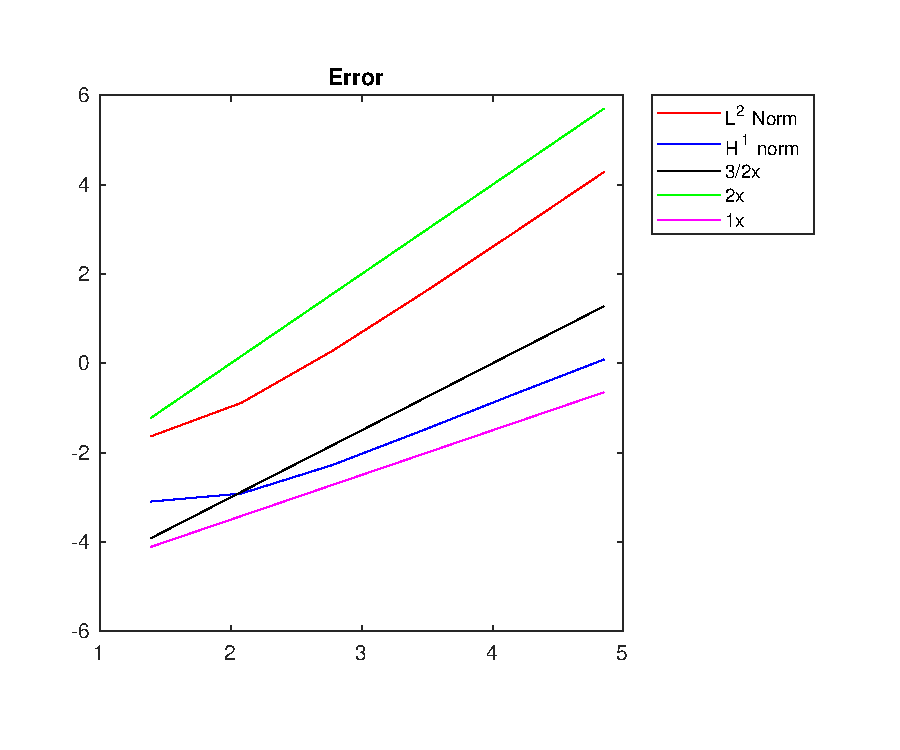
\includegraphics[width=10cm]{fig_dirichlet_error_G2_CP1_I1_M6_C2}
		%%\caption{fig dirichlet error G2 CP1 I1 M6 C2}
	\end{figure}
	\noindent$\bullet$ \underline{Case 3:}
	\begin{figure}[H]
		\centering	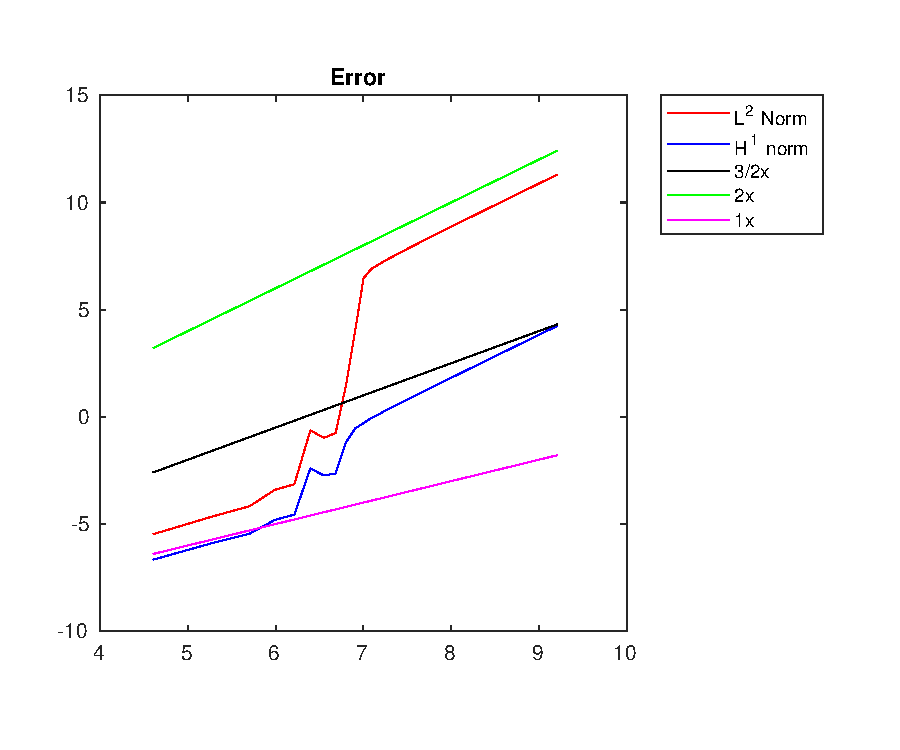
\includegraphics[width=10cm]{fig_dirichlet_error_G2_CP1_I1_M100_C3}
		%%\caption{fig dirichlet error G2 CP1 I1 M100 C3}
	\end{figure}
	\noindent\textbf{Remark:}\\
	In case 1, the method appears to have convergence rate of order $2$ in $L^2$ norm and order $\frac{3}{2}$ in energy norm.\\
	In case 2, the method appears to have convergence rate of order $2$ in $L^2$ norm and order $1$ in energy norm.\\
	In case 3, the method appears to have convergence rate of order $2$ in both $L^2$ energy norm and there are some "irregularities" in the convergence rate before the grid refinement reach a certain degree.\\

	\newpage

	\section{Neumann boundary condition}
	In this section, we are going to test the Finite Volume Method for the 1-dimensional Poisson equation subjected to Neumann boundary condition with several test cases using uniform grid and singular grid.
	\subsection{Main idea}
	We now review the problem we need to solve
	\begin{flalign}
	-u''(x)&=f(x), x\in\Omega &\\
	u'(0)&=0 &\\
	u'(1)&=0 &\\
	\int_{0}^{1}f(x)dx&=0 &\\
	\int_{0}^{1}u(x)dx&=0 \label{intu0}&
	\end{flalign}
	We note that if we omit the condition \eqref{intu0}, this problem will have infinitely many solutions of the form $u_1(x)+c$, with $u_1(0)$ being a solution of the problem.\\
	Let $\left[U_0, U_1, U_2, \dots,U_N, U_{N+1}\right]^\intercal$ be the discrete solution of the problem.\\
	When using derivative approximation with first order convergence rate, the boundary condition can be "discretized" as $U_0=U_1$ and $U_N=U_{N+1}$. Then, we need to use the linear system to solve for $U=\left[U_1, U_2, \dots,U_N\right]^\intercal$\\
	We also note that the discretized linear system has 1 independent variable. Therefore, we can choose to solve for one solution $\bar{U}$ such that $U_K=0$ for some $K$ and then use the condition $\int_{0}^{1}u(x)dx=0$ to find the constant $C$ such that $U=\bar{U}+C$ satisfies the condition.\\

	\subsection{Test cases}
	\noindent$\bullet$ \underline{Case 1:}
	\begin{flalign*}
	f(x)&=\frac{1}{2}-x&\\
	\int_{0}^{1}f(x)&=0&\\
	u'(0)&=0&\\
	u'(1)&=0&\\
	u(x)&=\frac{x^2\,\left(2\,x-3\right)}{12}+\frac{1}{24}&\\
	\int_{0}^{1}u(x)&=0
	\end{flalign*}

	\noindent$\bullet$ \underline{Case 2:}
	\begin{flalign*}
	f(x)&=400\pi^2\cos\left(20\pi x\right)&\\
	\int_{0}^{1}f(x)&=0&\\
	u'(0)&=0&\\
	u'(1)&=0&\\
	u(x)&=\sin\left(20\pi x +\frac{\pi}{2}\right)&\\
	\int_{0}^{1}u(x)&=0
	\end{flalign*}

	\newpage
	\subsection{Homogeneous Neumann boundary condition, regular grid, each control point is the midpoint of corresponding control volume, integration using midpoint rule}
	\subsubsection{Figures of results}
	\noindent$\bullet$ \underline{Case 1:}
	\begin{figure}[H]
		\centering	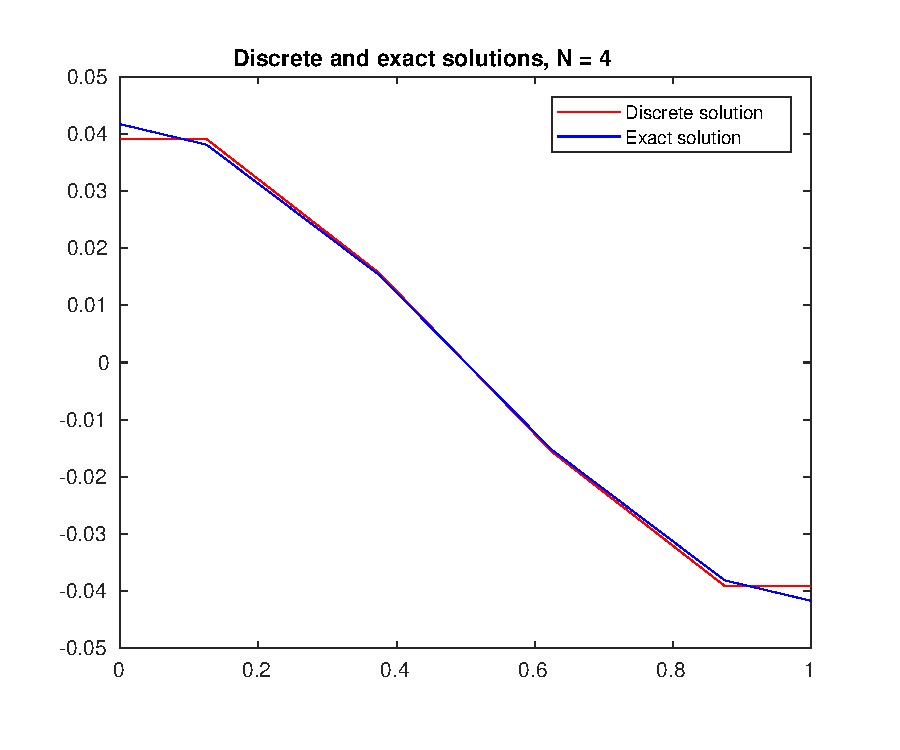
\includegraphics[width=10cm]{fig_neumann_result_G1_CP1_I1_N4_M6_C1}
		%%\caption{fig neumann result G1 CP1 I1 N4 M6 C1}
	\end{figure}
	\begin{figure}[H]
		\centering	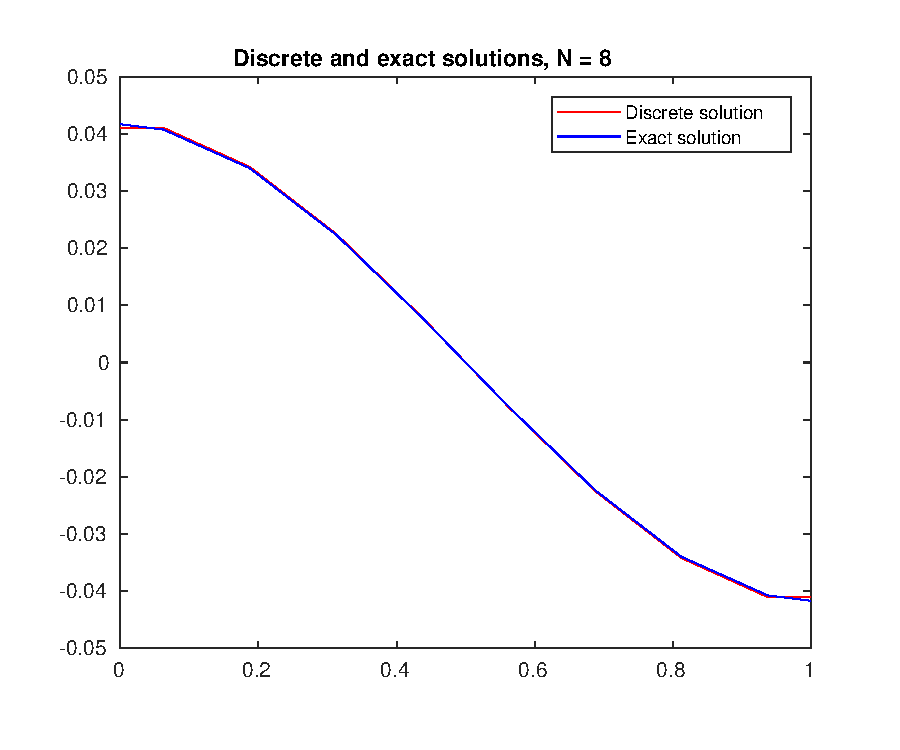
\includegraphics[width=10cm]{fig_neumann_result_G1_CP1_I1_N8_M6_C1}
		%%\caption{fig neumann result G1 CP1 I1 N8 M6 C1}
	\end{figure}
	\begin{figure}[H]
		\centering	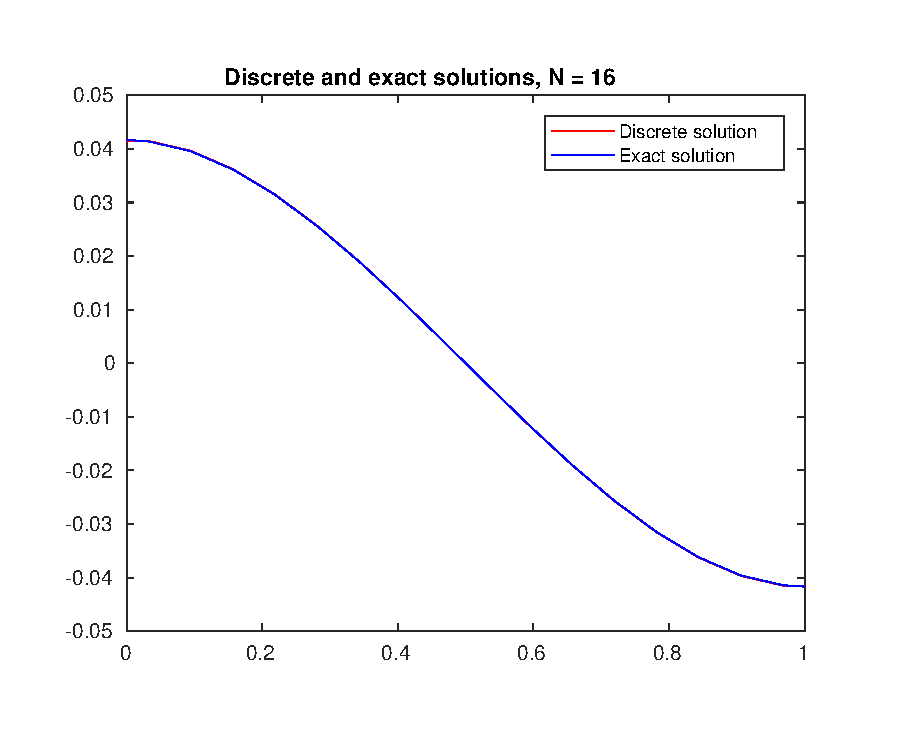
\includegraphics[width=10cm]{fig_neumann_result_G1_CP1_I1_N16_M6_C1}
		%%\caption{fig neumann result G1 CP1 I1 N16 M6 C1}
	\end{figure}
	\begin{figure}[H]
		\centering	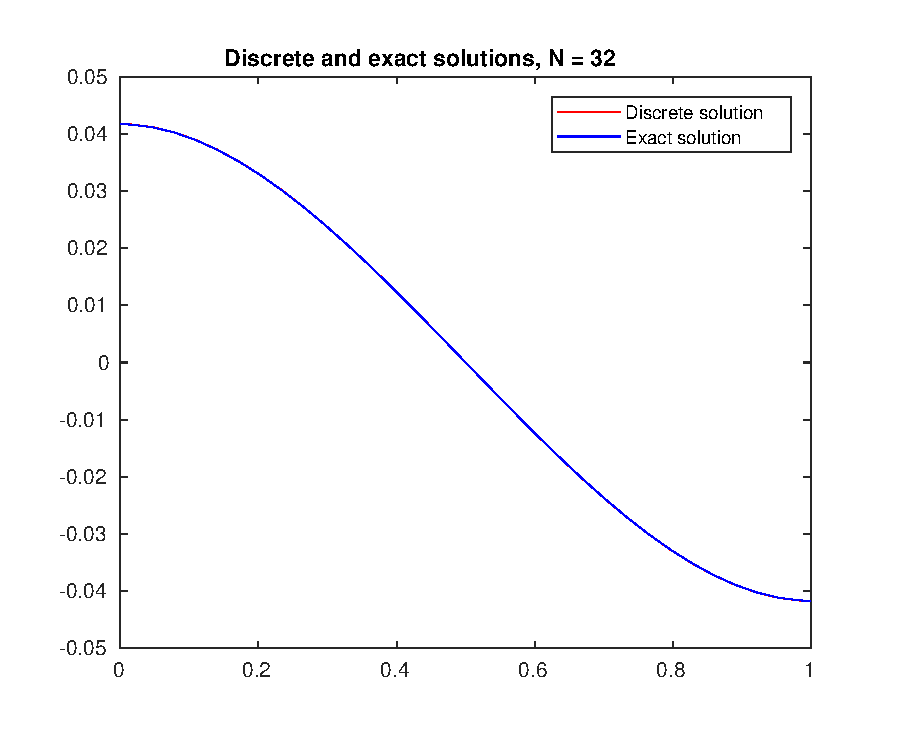
\includegraphics[width=10cm]{fig_neumann_result_G1_CP1_I1_N32_M6_C1}
		%%\caption{fig neumann result G1 CP1 I1 N32 M6 C1}
	\end{figure}
	\begin{figure}[H]
		\centering	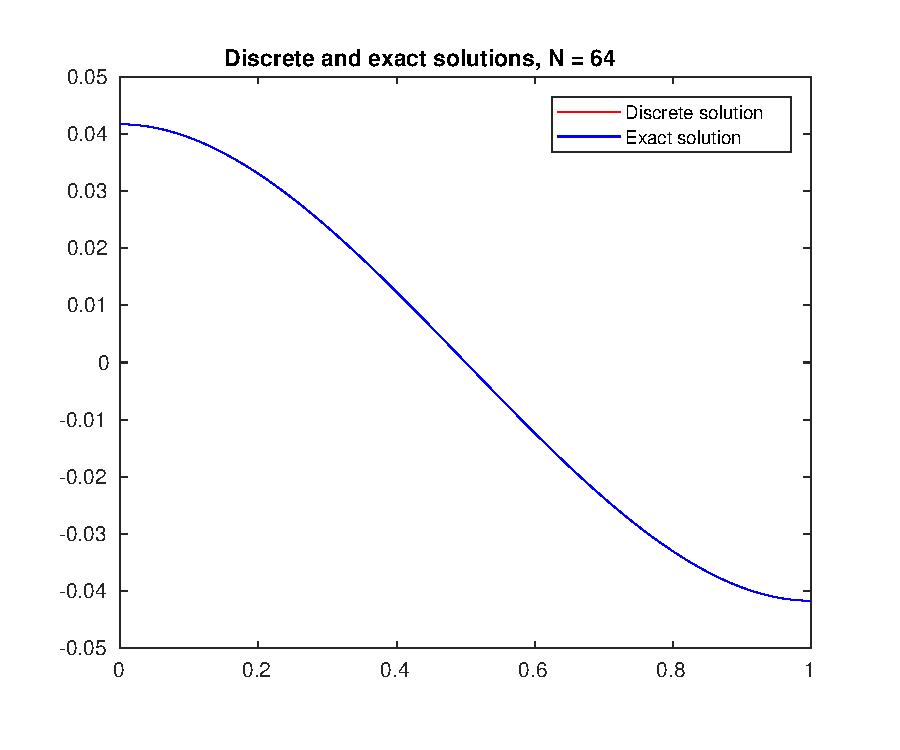
\includegraphics[width=10cm]{fig_neumann_result_G1_CP1_I1_N64_M6_C1}
		%%\caption{fig neumann result G1 CP1 I1 N64 M6 C1}
	\end{figure}
	\begin{figure}[H]
		\centering	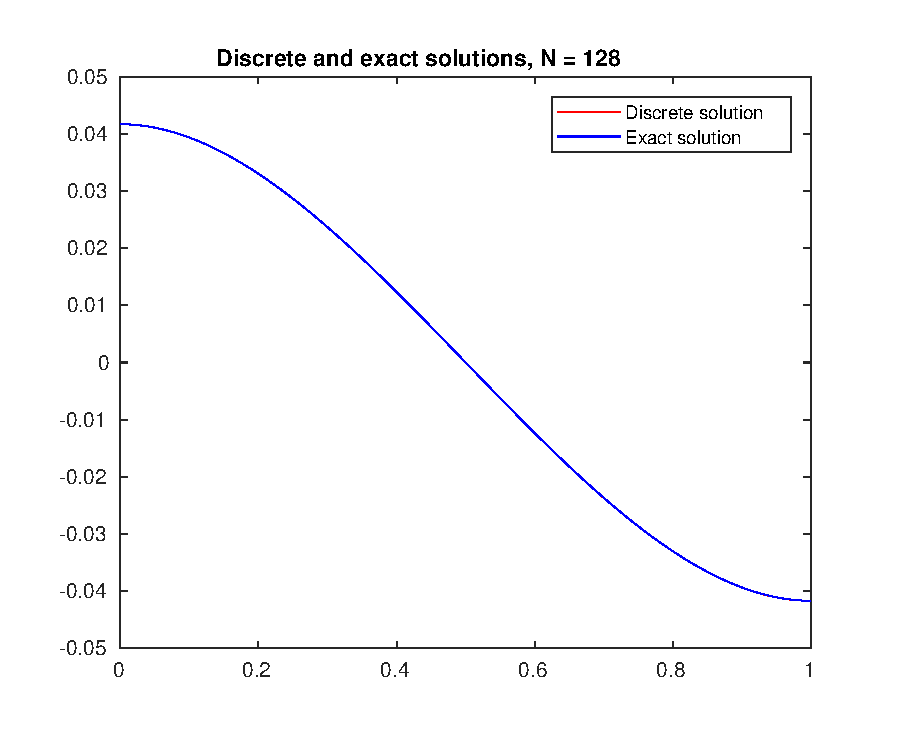
\includegraphics[width=10cm]{fig_neumann_result_G1_CP1_I1_N128_M6_C1}
		%%\caption{fig neumann result G1 CP1 I1 N128 M6 C1}
	\end{figure}

	\noindent$\bullet$ \underline{Case 2:}
	\begin{figure}[H]
		\centering	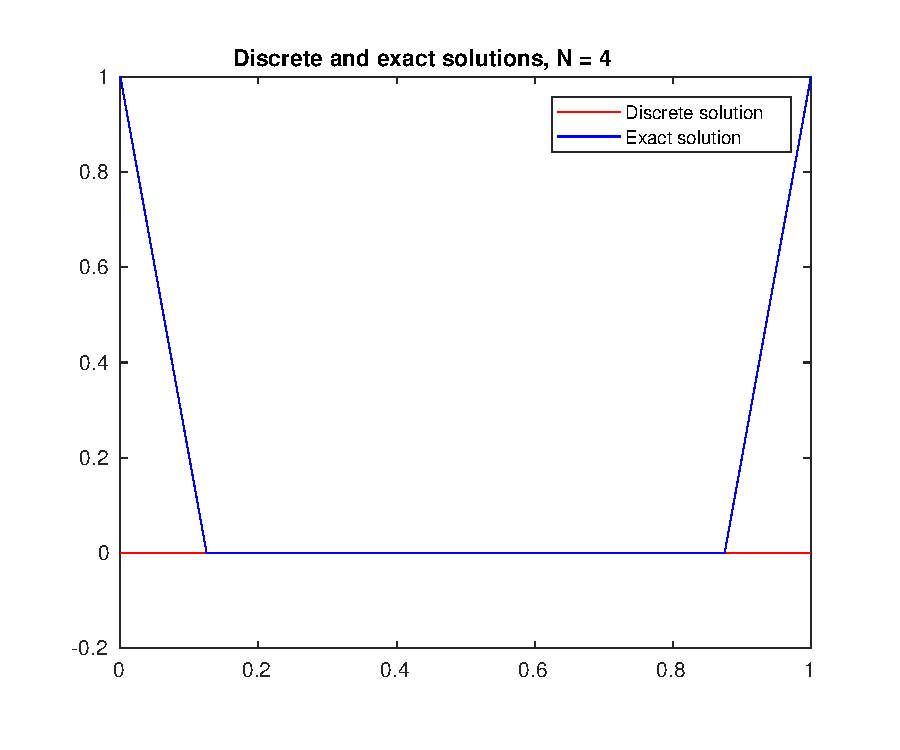
\includegraphics[width=10cm]{fig_neumann_result_G1_CP1_I1_N4_M6_C2}
		%%\caption{fig neumann result G1 CP1 I1 N4 M9 C2}
	\end{figure}
	\begin{figure}[H]
		\centering	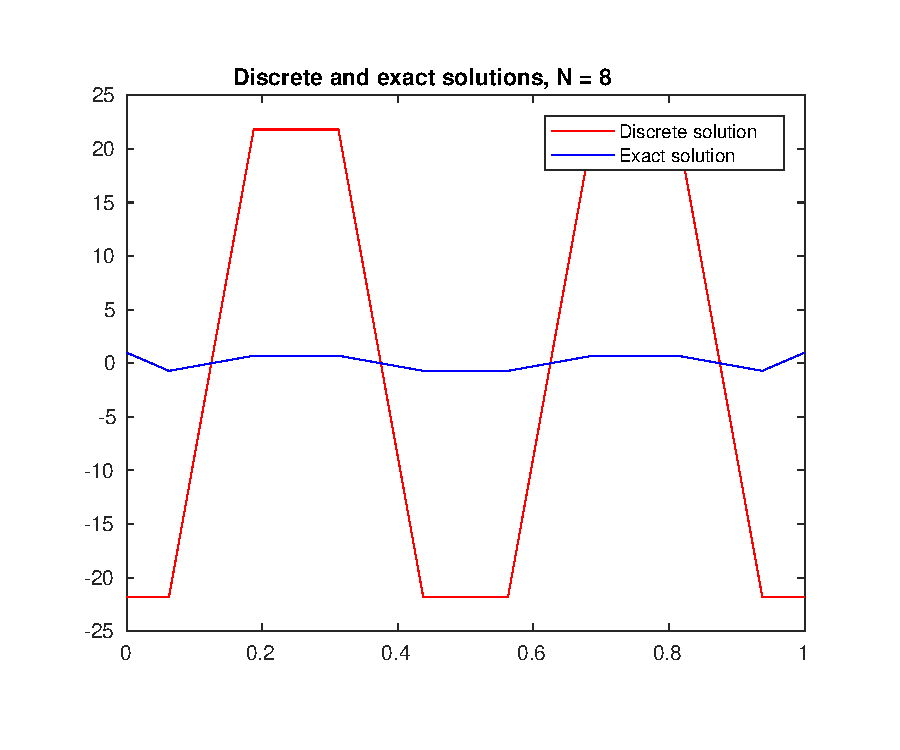
\includegraphics[width=10cm]{fig_neumann_result_G1_CP1_I1_N8_M6_C2}
		%%\caption{fig neumann result G1 CP1 I1 N8 M9 C2}
	\end{figure}
	\begin{figure}[H]
		\centering	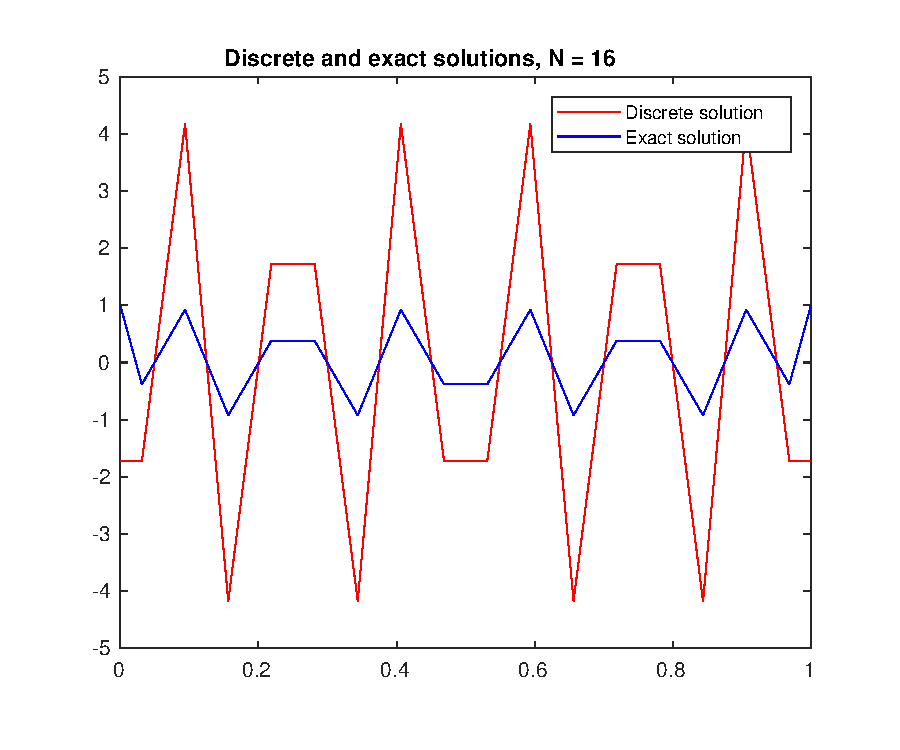
\includegraphics[width=10cm]{fig_neumann_result_G1_CP1_I1_N16_M6_C2}
		%%\caption{fig neumann result G1 CP1 I1 N16 M9 C2}
	\end{figure}
	\begin{figure}[H]
		\centering	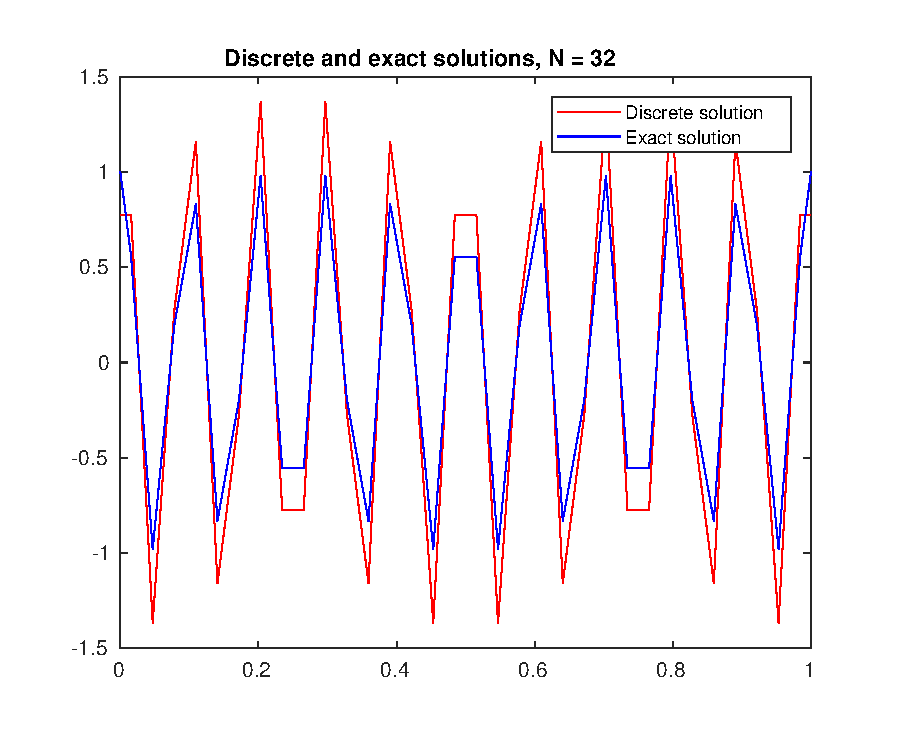
\includegraphics[width=10cm]{fig_neumann_result_G1_CP1_I1_N32_M6_C2}
		%%\caption{fig neumann result G1 CP1 I1 N32 M9 C2}
	\end{figure}
	\begin{figure}[H]
		\centering	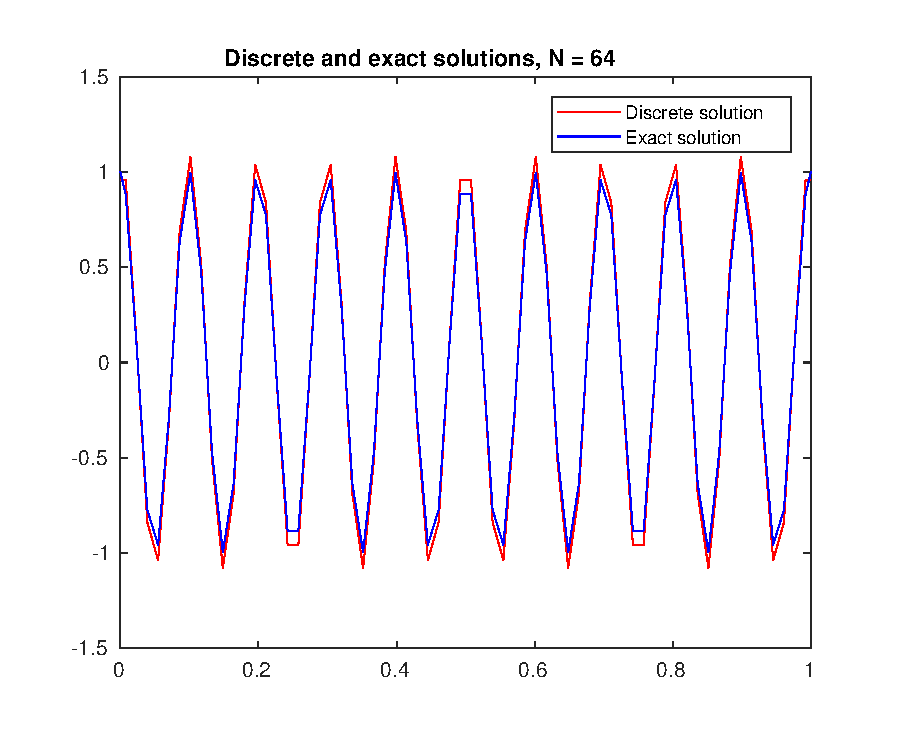
\includegraphics[width=10cm]{fig_neumann_result_G1_CP1_I1_N64_M6_C2}
		%%\caption{fig neumann result G1 CP1 I1 N64 M9 C2}
	\end{figure}
	\begin{figure}[H]
		\centering	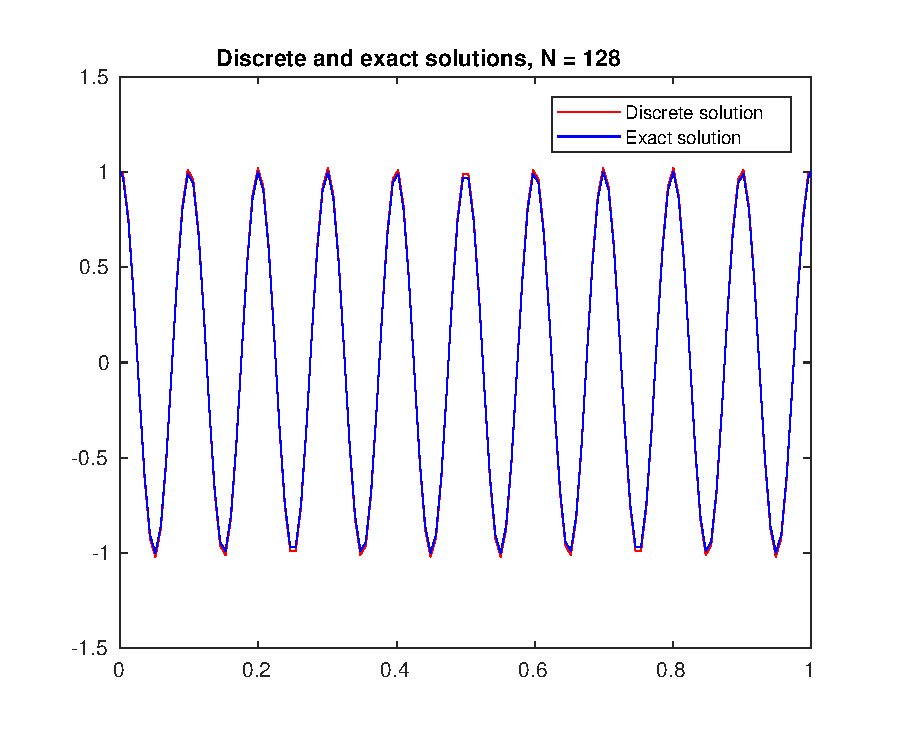
\includegraphics[width=10cm]{fig_neumann_result_G1_CP1_I1_N128_M6_C2}
		%%\caption{fig neumann result G1 CP1 I1 N128 M9 C2}
	\end{figure}
	\begin{figure}[H]
		\centering	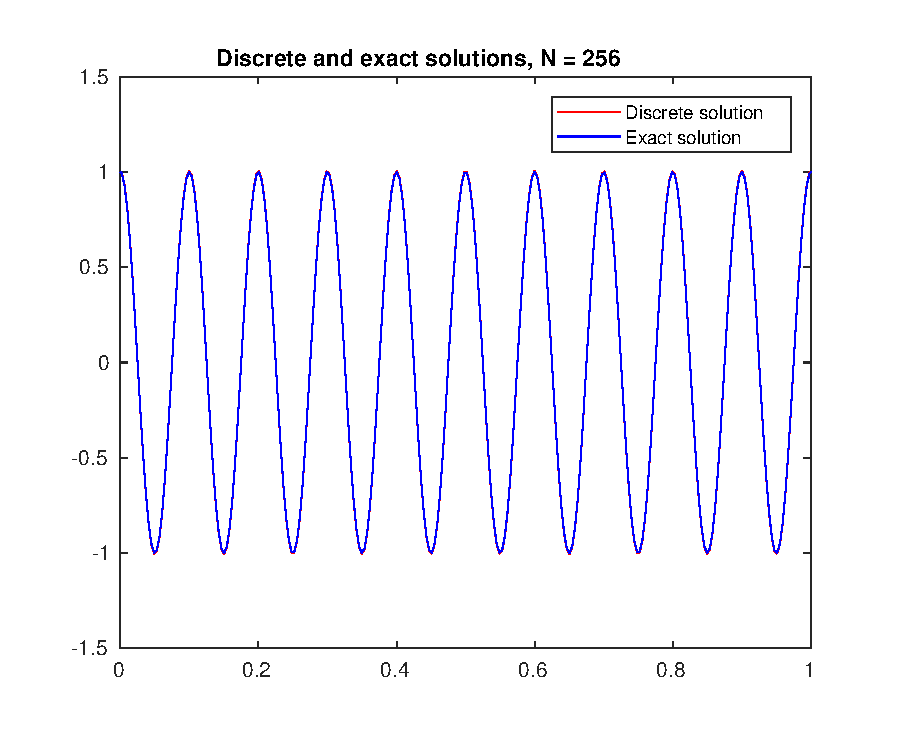
\includegraphics[width=10cm]{fig_neumann_result_G1_CP1_I1_N256_M9_C2}
		%%\caption{fig neumann result G1 CP1 I1 N256 M9 C2}
	\end{figure}
	\begin{figure}[H]
		\centering	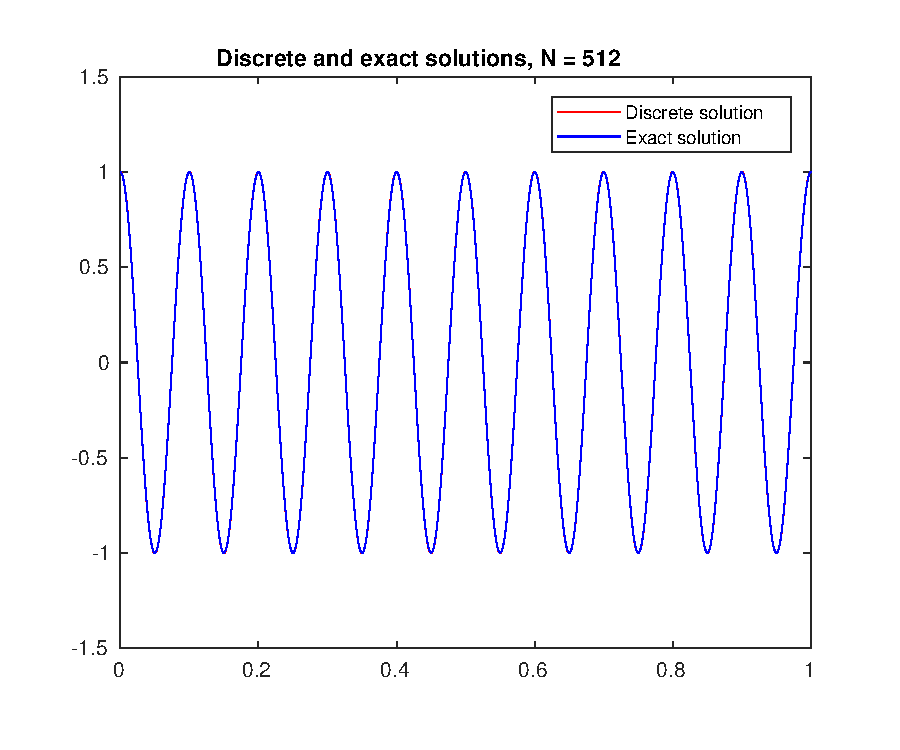
\includegraphics[width=10cm]{fig_neumann_result_G1_CP1_I1_N512_M9_C2}
		%%\caption{fig neumann result G1 CP1 I1 N512 M9 C2}
	\end{figure}
	\begin{figure}[H]
		\centering	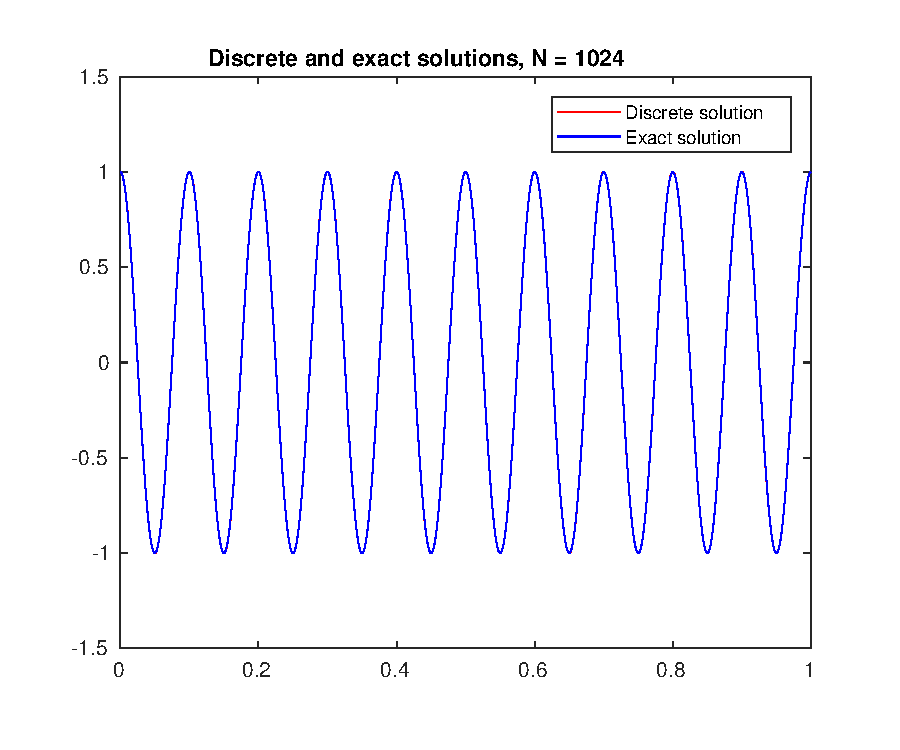
\includegraphics[width=10cm]{fig_neumann_result_G1_CP1_I1_N1024_M9_C2}
		%%\caption{fig neumann result G1 CP1 I1 N1024 M9 C2}
	\end{figure}
	\subsubsection{Errors}
	\noindent$\bullet$ \underline{Case 1:}
	\begin{table}[H]
		\centering
		\begin{tabu}{|c|c|c|}
			\hline
			N	&  $\lVert u_{discrete}-u_{exact}\rVert_{L^2}$& $\lVert u_{discrete}-u_{exact}\rVert_{H^1}$ \\\hline
			4	& 7.278867e-04 & 1.449939e-02 \\\hline
			8	& 1.864655e-04 & 5.329006e-03 \\\hline
			16	& 4.689303e-05 & 1.918917e-03 \\\hline
			32	& 1.174048e-05 & 6.845135e-04 \\\hline
			64	& 2.936197e-06 & 2.430787e-04 \\\hline
			128	& 7.341164e-07 & 8.612922e-05 \\\hline
		\end{tabu}
		%%\caption{Error table}
	\end{table}

	\noindent$\bullet$ \underline{Case 2:}
	\begin{table}[H]
		\centering
		\begin{tabu}{|c|c|c|}
			\hline
			N	&  $\lVert u_{discrete}-u_{exact}\rVert_{L^2}$& $\lVert u_{discrete}-u_{exact}\rVert_{H^1}$ \\\hline
			4	& 3.446145e-13 & 4.000000e+00 \\\hline
			8	& 2.110184e+01 & 2.389353e+02 \\\hline
			16	& 2.486740e+00 & 7.434583e+01 \\\hline
			32	& 2.787005e-01 & 1.565996e+01 \\\hline
			64	& 5.963946e-02 & 4.064360e+00 \\\hline
			128	& 1.437125e-02 & 1.122033e+00 \\\hline
			256	& 3.560351e-03 & 3.281879e-01 \\\hline
			512	& 8.880771e-04 & 1.017972e-01 \\\hline
			1024	& 2.218939e-04 & 3.318688e-02 \\\hline
		\end{tabu}
		%%\caption{Error table}
	\end{table}

	\noindent\textbf{Remark:}
	\newpage
	\subsubsection{Convergence rate}
	\noindent$\bullet$\underline{Case 1:}
	\begin{figure}[H]
		\centering	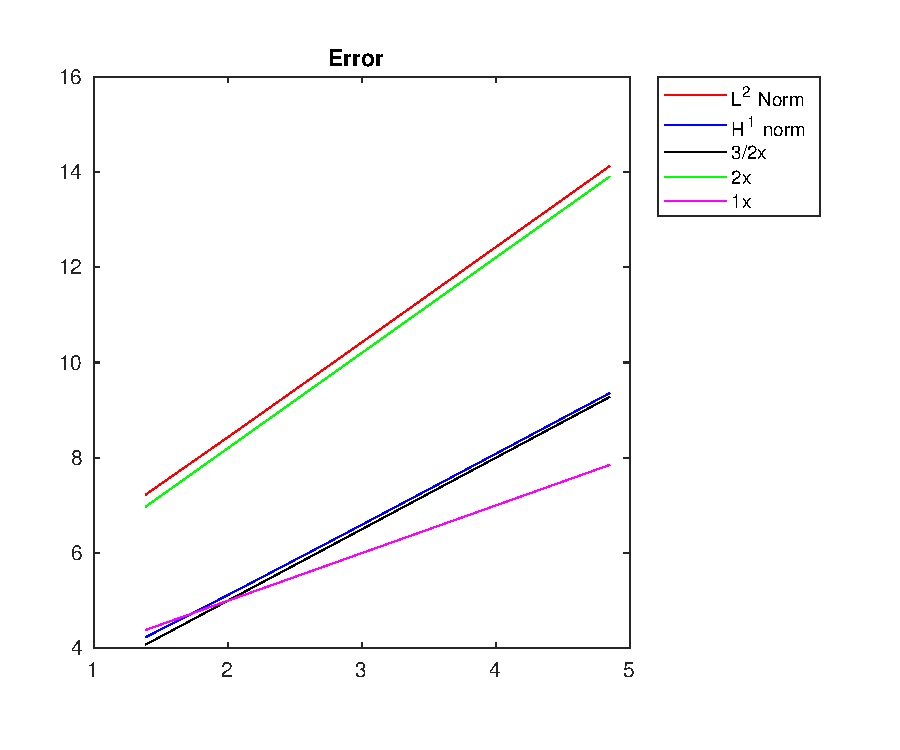
\includegraphics[width=10cm]{fig_neumann_error_G1_CP1_I1_M6_C1}
		%%\caption{fig neumann error G1 CP1 I1 M6 C1}
	\end{figure}
	\noindent$\bullet$\underline{Case 2:}
	\begin{figure}[H]
		\centering	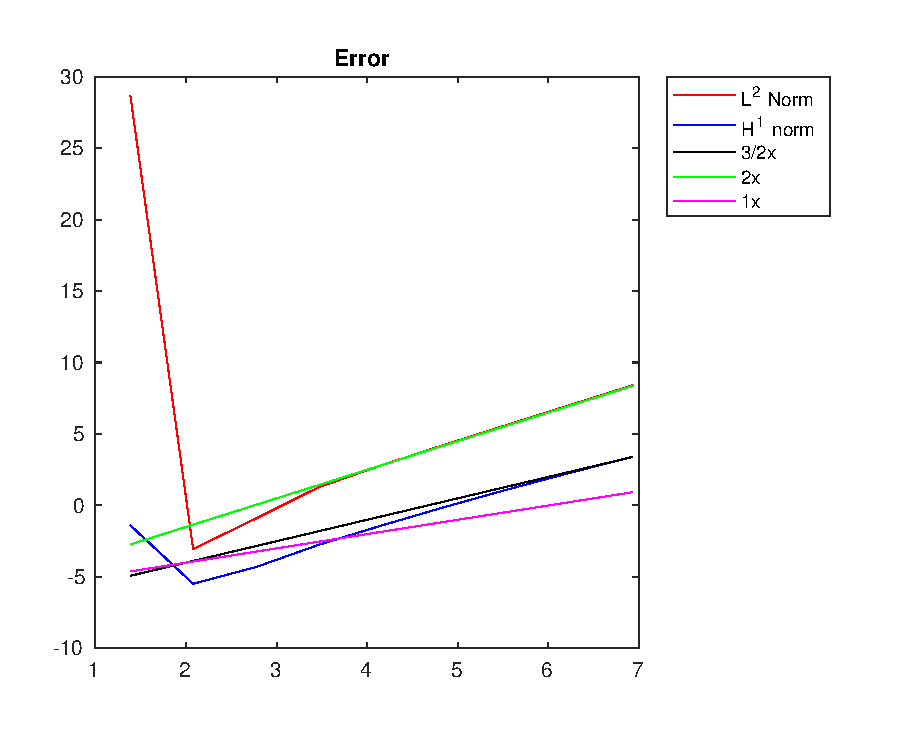
\includegraphics[width=10cm]{fig_neumann_error_G1_CP1_I1_M9_C2}
		%%\caption{fig neumann error G1 CP1 I1 M9 C2}
	\end{figure}
	\noindent\textbf{Remark:} In both case 1 and 2, the method appears to have convergence rate of order $2$ in $L^2$ norm and order $\frac{3}{2}$ in energy norm.
	\newpage

	\subsection{Homogeneous Neumann boundary condition, singular grid, each control point is the midpoint of corresponding control volume, integration using midpoint rule}
	Again, we will consider the grid $x_i=1-\cos\left(\frac{\pi i}{2(N+1)}\right)$ in this section.
	\subsubsection{Errors}
	\noindent$\bullet$ \underline{Case 1:}
	\begin{table}[H]
		\centering
		\begin{tabu}{|c|c|c|}
			\hline
			N	&  $\lVert u_{discrete}-u_{exact}\rVert_{L^2}$& $\lVert u_{discrete}-u_{exact}\rVert_{H^1}$ \\\hline
			4	& 4.300279e-03 & 2.361702e-02 \\\hline
			8	& 4.473365e-04 & 7.452580e-03 \\\hline
			16	& 7.886546e-05 & 2.530245e-03 \\\hline
			32	& 1.995312e-05 & 9.154423e-04 \\\hline
			64	& 5.129577e-06 & 3.310069e-0 \\\hline
			128	& 1.302358e-06 & 1.185516e-04 \\\hline
		\end{tabu}
		%%\caption{Error table}
	\end{table}

	\noindent$\bullet$ \underline{Case 2:}
	\begin{table}[H]
		\centering
		\begin{tabu}{|c|c|c|}
			\hline
			N	&  $\lVert u_{discrete}-u_{exact}\rVert_{L^2}$& $\lVert u_{discrete}-u_{exact}\rVert_{H^1}$ \\\hline
			4	& 2.518759e+02 & 8.229286e+02 \\\hline
			8	& 2.924364e+01 & 2.378888e+02 \\\hline
			16	& 9.888043e+01 & 3.764880e+02 \\\hline
			32	& 5.525841e-01 & 2.551420e+01 \\\hline
			64	& 1.099226e-01 & 6.825063e+00 \\\hline
			128	& 2.584269e-02 & 1.840590e+00 \\\hline
			256	& 6.388832e-03 & 5.196868e-01 \\\hline
			512	& 1.595856e-03 & 1.549021e-01 \\\hline
			1024	& 3.992680e-04 & 4.880113e-02 \\\hline
		\end{tabu}
		%%\caption{Error table}
	\end{table}

	\noindent\textbf{Remark:}
	\newpage
	\subsubsection{Convergence rate}
	\noindent$\bullet$\underline{Case 1:}
	\begin{figure}[H]
		\centering	\includegraphics[width=10cm]{fig_neumann_error_G2_CP1_I1_M6_C1}
		%%\caption{fig neumann error G2 CP1 I1 M6 C1}
	\end{figure}
	\noindent$\bullet$\underline{Case 2:}
	\begin{figure}[H]
		\centering	\includegraphics[width=10cm]{fig_neumann_error_G1_CP1_I1_M9_C2}
		%%\caption{fig neumann error G2 CP1 I1 M9 C2}
	\end{figure}
	\noindent\textbf{Remark:} In both case 1 and 2, the method appears to have convergence rate of order $2$ in $L^2$ norm and order $\frac{3}{2}$ in energy norm.
	\newpage
\end{document}
